%
\documentclass{article}
\usepackage{geometry}
\usepackage{url}
\geometry{a4paper, margin=2cm}

\usepackage{times,graphicx,amsfonts}
\usepackage{algorithm}
\usepackage{algorithmicx}
\usepackage[tbtags]{amsmath}
\usepackage{cases}
\usepackage{array}
\usepackage{algpseudocode}
\usepackage{amsmath}
\usepackage{graphics}
 \usepackage{graphicx}
\usepackage{url}
\usepackage[T1]{fontenc}
\usepackage{amssymb}
\usepackage{cite}
\usepackage{mathrsfs}
\usepackage{caption}
\usepackage{subfigure}
\usepackage{ulem}
\usepackage{multirow}
\usepackage{textcomp}
\usepackage{stfloats}
\usepackage{diagbox}

%%%%%%%%%%%%%%%%%%%%%

\DeclareCaptionLabelSeparator{dot twospace}{.  } \captionsetup{labelsep=dot twospace}
\newcommand{\systemname}{SLEEPGUARD}
\newtheorem{assump}{Assumption}
\newtheorem{axiom}{Axiom}
\newtheorem{claim}{Claim}
\newtheorem{conj}{Conjecture}[section]
\newtheorem{crit}{Criterion}
\newtheorem{theorem}{Theorem}
\newtheorem{coro}{Corollary}[theorem]
\newtheorem{definition}{Definition}
\newtheorem{example}{Example}
\newtheorem{fact}{Fact}
\newtheorem{hypo}{Hypothesis}
\newtheorem{lemma}{Lemma}
\newtheorem{obsv}{Observation}[theorem]
\newtheorem{prin}{Principle}
\newtheorem{prob}{Problem}
\newtheorem{ppty}{Property}
\newtheorem{propo}{Proposition}
\newtheorem{protocol}{Protocol}
\newtheorem{remark}{Remark}
\newtheorem{test}{Test}
\newtheorem{transform}{Conversion Algorithm}
\newcommand{\tabincell}[2]{\begin{tabular}{@{}#1@{}}#2\end{tabular}}

\renewcommand{\algorithmicrequire}{\textbf{Input:}}
\renewcommand{\algorithmicensure}{\textbf{Output:}}
\usepackage{color}

\newcommand{\ignore}[1]{{}}
\usepackage{makeidx}
\makeindex

\hfuzz=\maxdimen \tolerance=10000 \hbadness=10000

\newcommand\FIXME[1]{\textcolor{red}{FIX:}\textcolor{red}{#1}}


%\bibliographystyle{ACM-Reference-Format}

\begin{document}

{\large\noindent \textbf{Respond to reviewers' comments -- Capturing Rich Sleep Information using Smartwatch Sensing Data}
\\
}

\vspace{10mm}

 \noindent{Dear Editor,}

\vspace{10mm}

We thank the reviewers for their constructive feedback. In the revised manuscript, we have tried to address all the issues raised by the
reviewers. Please find attached to this letter a summary of the major changes and  detailed responses to each reviewer.

\vspace{10mm}

\noindent{Sincerely yours,}\\

\vspace{5pt}

\noindent{Liqiong Chang}




%%%%%%%%%%%%%%%%%%%%%%%%%%%%%%%%%%%%%%%%%%%%%%%%%%%%%%%%%
\noindent\rule{\textwidth}{1pt}

\section*{List of Major Changes}

Here we respond to the main comments, noting which reviews they come from.

\paragraph{M1.} We have better highlighted the motivation and scientific contributions of the work in Section 1.1 and demonstrated that how our work can lead to
a better understanding of the sleep quality in Section 4.2.4. In particular, we show that users valued the additional information extracted by our system, and that capturing this information enabled our system to identify reasons for suboptimal sleep quality. 

\paragraph{M2.} We have clarified the aim and better explained the results of our user survey, showing how \systemname can help users
improve their sleep behaviours (a question raised by all reviewers). This can be found at Section 4.2.4. The revision shows that
\systemname successfully helped some of our testing users in understanding the causes of poor sleeps. Specifically, our data reveal that
the hand position was the reason for frequent numb arms and nightmares for two of our participants, the sleeping posture and hand position
contributed to snoring for another participant, and the excessive light intensity and frequent noises of the environment led to bad sleeps
for a fourth participant. These four users correspond to the set of (four) users that rated their subjective sleep quality as bad in our experiment. Additionally, two users rated their sleep quality as general, but for these users no clear reason were found. Based on these findings, we then suggested ways to improve their sleeping habits and a return visit of these
users shows that our suggestions helped to improve their sleep quality. 

\paragraph{M3.} We now provide discussions on the use of a PSG in Sections 1 and 6 (a question raised by reviewers 1 and 4). See also R1.1.

\paragraph{M4.} Section 2.1 and Section 3.1 of the revised manuscript give further details on our experimental setup per reviewer feedback (raised by reviewers 1, 4 and 5). See also R1.2, R1.4, R4.4, R4.6, and R5.11.

\paragraph{M5.} We have updated Section 2.4 to include a detailed description of our Hidden Markov Model (HMM) model (raised by reviewers 1 and 4). See also R1.5.


\paragraph{M6.} We have provided a discussion on how to tackle multiple-sleeper scenarios, the occurrence of unusual arm positions, etc. This can be
found at Section 5.

\paragraph{M7.} We have made all the minor corrections suggested by the reviewers and some others.


\newpage
%\noindent\rule{\textwidth}{1pt}
%
%\vspace{2mm}
\section*{Detailed Responses}

\noindent We now give our detailed responses for each reviewer.

\section*{Reviewer 1}

\paragraph{R1.1} We have extended the introduction to discuss the advantages and disadvantages of PSG and why it is not applicable to our
problem. Thanks for the comments.

\paragraph{R1.2} Embarrassed not to have introduced and provided sufficient details on our pilot study. This information is now given in Section 3.

\paragraph{R1.3} We take 12-28 samples every minute to detect respiratory events. This is based on the observation that an adult typically
breathes around 15 times per minute. We found that this setting is effective for our problem. This is now clarified in Section 2.1.

\paragraph{R1.4} The 10 volunteers involved in the training data process (pilot study) for determining the algorithm parameters are different from the 15 users recruited in our
evaluation. The data were collected while they were sleeping. This is clarified in Section 2.1 in the revised manuscript.

\paragraph{R1.5} Our HMM model is trained using the training data. This is now clarified in Section 2.4. See also R1.4.
\vspace{-2mm}
\paragraph{R1.6} To evaluate our approach, we have randomly picked at least 3 sets of data from each of our 15 testing users.
The current submission is not evaluated on the full dataset (videos of a over 1,000 hours) due to the time constraint (as we need to watch
each video to mark sleep events). That said, we are able to demonstrate the usefulness of our approach on a relatively small but
representative set of data. We are currently working to extend our evaluation to the entire dataset. The results will be ready for and
included in the camera ready paper.

\paragraph{R1.7} ``invasive" is indeed a poorly chosen word for describing Fibit. We have reworded.
\vspace{-2mm}
\paragraph{R1.8} The signals shown in Fig.5 are from a single subject. This is clarified in the revised version.

\paragraph{R1.9} Our work monitors the changes of speeds caused by respiration, which is then used to detect the relevant respiratory events.
While our approach is effective when the hand is put on the chest, we observe little changes in the speeds when the hand is put on the
shoulder (which makes it difficult to accurately detect respiratory motions). We have extended Section 2.1 in the revised version with new
data to explain this. Thanks for the feedback.

\paragraph{R1.10} Good catch, the sentence should be instead read as ``A body rollover event is recorded when the posture changes are detected between
two time points". We have now corrected the phrase.

\paragraph{R1.11} We have given the parameters for the moving average filter and explain how they are obtained in Section 2.1 in the revised version.

\paragraph{R1.12} The acceleration threshold was determined from our training data. This is now clarified in Section 2.1. See also
R1.4.

\vspace{-2mm}
\paragraph{R1.13} Our algorithm does consider a situation where the wrist turns so that the back of the hand become downward. This is now clarified in Section 2.3.

\paragraph{R1.14} Yes, there is no standard definition for sleep stages. We have provided our definitions of the various stages (per reviewer suggestions) in Section 2.4.

\paragraph{R1.15} We have extended Section 5 to discuss how our approach can be extended to a multi-sleeper scenario.

\paragraph{R1.16} The ground truth of micro-body movements are obtained through (a) watching videos and (b) using the phone accelerometer data. We use the accelerometer data is because visions of subtle body movements may be blocked due to camera angles or surrounding objects e.g., quilt. This is clarified in Section 4.1.4.

\paragraph{R1.17} We have provided a more detailed analysis and discussion for Table 9 in Section 4.2.4.

\paragraph{R1.18} Having a discussion on the frequency of unusual arm positions is a great point. This is now included in Section 5.

\paragraph{R1.19} We have make all the minor corrections and fixed the presentation issues. Many thanks for the feedback.

\section*{Reviewer 2}
\paragraph{R2.1} Our work focuses more on tracking sleep behaviours (like hand positions and respiratory motions) and the sleeping environment (like lighting and acoustic events), but not sleep stages. Our goal is to help a user to understand poor sleep but not quantify the sleep quality. We do not compare to medical-grade equipment like PSG due to the scope of the work and for practical reasons (please see also R4.1 and R1.1). Thanks for the feedback.


\paragraph{R2.2} Yes, \systemname is a sleep monitoring system for wearable devices. However, it can track a richer set of events
(including body postures, hand positions, body rollover counts, micro-body movements, and acoustic events) that are not supported by
Fitbit. We show that these rich events can help some of our users in understanding the causes of poor sleep and subsequently to improve
their sleep quality (see also M2). We have revised the introduction section to better highlight our contributions. Thanks for the feedback.

\paragraph{R2.3} Our paper presents new algorithms to monitor and detect a range of sleep activities (like body postures, hand positions,
micro-body movements etc.) on wearable devices. Many of these are not supported by Fitbit, a state-of-the-art sleep monitoring system on
wearable devices. We also demonstrate that the tracked events can help users improve their sleep quality. This contribution is now
highlighted in Section 1.

\section*{Reviewer 3}
\paragraph{R3.1} We agree that the discussion and analysis of the user survey should be improved. As such, we have extended Section 4.2.4
in the revised version with new analysis, evidences and discussions, showing how \systemname helps some of our participants in
understanding the cause of poor sleeps and in taking actions to improve their sleeps. Please see also M2.

\paragraph{R3.2} Agree that evidence should be provided to demonstrate the benefit of \systemname. Such information is given in Section
4.2.4. Compared to medical equipment like PSG, which tracks physiological signals, such as brain waves and electrocardiogram, the sleep
events given by \systemname, such as postures, hand positions, body movements etc., can be more easily understood by people who have no
medical background. Much of such information is not provided by Fitbit, the state-of-art commercial-grade sleep monitoring system for
wearable devices. Please see also M2 on how \systemname help our users understand and improve their sleep behaviours.

\section*{Reviewer 4}

\paragraph{R4.1} We agree with the reviewer that it would be interesting to compare our work against a PSG if possible. However, doing so
is infeasible because of the focus of the work and practical reasons. Our work focuses on tracking a user's physical activities (like hand
positions and body rollover) and the sleeping environment (like lighting and acoustic events), and we need to achieve these with as little
disruption to the user's normal sleep as possible. A PSG would only track the user's sleep stages. It is not only expensive to buy, but
will also cause significant disruptions to a user's normal sleep. These make it difficult to perform a large-scale experiment across a
long-period of time using PSGs. Instead, we choose to compare our work with Fitbit as its accuracy is shown to be comparable to a PSG.
However, we show that our approach can track more events and lead to a better understand of the sleep quality than Fitbit. We have
clarified and provided a discussion on this in \FIXME{Section xx}. Please see also R4.3. We thank the reviewer for the feedback.

\paragraph{R4.2} We have performed further analysis on our user study per the review feedback. Please refer to M2. We have also reworded our
claims. Thank you.


\paragraph{R4.3} We have provided a discussion on the advantages and disadvantages for PSG in \FIXME{Section xx}. See also R1.1. Thanks for the feedback.

\paragraph{R4.4} Please see our response to R1.2 regarding our pilot study.

\paragraph{R4.4} Please refer to R1.3 on how the thresholds of respiration detection are chosen.

\paragraph{R4.5} The volunteers recruited for determining our algorithm parameters are different from those involved in
 evaluation. The details are provided in \FIXME{Section xx} of the revised manuscript. See also R1.4.

 \paragraph{R4.6} Please see our response to R1.5 on how the HMM model is built.

\section*{Reviewer 5}

\paragraph{R5.1} Compared to medical equipment, our approach is less intrusive and has less disruption for a user's sleep. The use of
single wrist sensors does have its limitations, because the hand movement frequency is different on different hands. However, such a
difference would only affect the detection of the hand position and micro movements, and can be largely cancelled through calibration. As
such, the limitation has little impact on understanding the sleep quality. This is explained at Section 5.


\paragraph{R5.2} Please see M2 on how our system help users to improve their sleep quality.

\paragraph{R5.3} We use multiple ways to establish our ground truths. These include watching and labelling video footage, compared to
Fitbit, and directly user involvement. Prior work has shown that Fitbit is accurately and effectively in tracking sleep stages, hence we use it to
establish some of our ground truths. Please see also R4.1.

\paragraph{R5.4} Yes, we are not the first to use wearable devices to track sleep behaviours. However, our work shows, for the first time, how
 to track a range of events using wearable devices, and how such information can help users to improve
their sleep behaviours. We have better highlighted our novelty in Section 6. Thanks for the feedback.

\paragraph{R5.5} Agree, in theory hands can be on any place. However, we found that the arm position strongly correlates to the body
posture. This allows us to effectively map the arm position to the sleeping posture. This is clarified in Sections 2.1.1 and 3.1 in the
revised manuscript.

\paragraph{R5.6} Our current implementation considers three hand positions as they are found to be the most common and representative
positions during our user study. However, our algorithms can be extended to other positions. This is explained at Section 2.1.2 in the new
version of the manuscript.

\paragraph{R5.7} The reviewer correctly pointed out that the breathing frequency can also be used to identify sleep stages. Our work uses
the respiratory amplitude which is strongly correlated to the breathing frequency, but the breathing frequency can also be used. This is
clarified at Section 4.2.2.

\paragraph{R5.8} We have extended the discussion of our hand position detection algorithm to provide more details in Section 2.1.2. We
thank the reviewer for the feedback.

\paragraph{R5.9} A large respiratory amplitude is defined as the average respiratory amplitude (15) of the
non-rapid-eye-movement (NREM) stage, and a normal respiratory amplitude is defined as the averaged respiratory amplitude (4) of the REM
stage. The definitions are based on the prior study [48] and our observation. This is now clarified in Section 2.1.2.


\paragraph{R5.10} The respiratory data collected in our training data are labeled using the following method. Our current implementation only detects
respiratory events when the hand is placed on the abnormal or the chest. The label of a sleep stage, i.e., REM or NREM, is confirmed when
both Fitbit and \systemname reach a consensus. We also watch the recorded video to label some large respiratory events if these are
observable from the video footage. Our classifier for respiratory events is k-nearest neighbor model (with $k=1$). This is now
clarified in Section 2.1.2.


\paragraph{R5.11} Our description for body rollover counts is wrong, sorry. We have fixed this error in the revised version. Please see
also R1.10.


\paragraph{R5.12} In Equation 7, \emph{x} and \emph{w} are the signal and impulse response respectively. We have clarified these in
Section 2.2.

\paragraph{R5.13} Compared to existing algorithms, our methods (equations 9-12) require less training data to build and hence incur less
data collection overhead. This is now clarified in Section 2.2.

\paragraph{R5.14} The parameters of Equations 11 and 12 were determined from our training data. This is clarified in Section 2.2. See also R1.4.

\paragraph{R5.15} Our illumination threshold was also chosen based on our training data -- we have visited the bedrooms of our 10 volunteers
to take the measurements using a light meter. We stress that this threshold can be adjusted without affecting the generalization ability of
our method. This is clarified in Section 2.3.

\paragraph{R5.16} There is no prior work on addressing the unstable light readings from smartwatches. The closest one is SleepHunter, a
smartphone-based approach. However, SleepHunter relies on the proximity sensor which is typically unavailable on smartwatches. This is
explained in Section 2.3.

\paragraph{R5.17} We have given the features used for sleep stage and quality measurement in Section 2.4 in the revised manuscript.
Specificially, we use four features, \#body rollers, \#micro-body movements, respiratory amplitudes, and \#acoustic events.

\paragraph{R5.18} The time window length is set to 15 minutes when no event is detected. However, when an event (e.g., the change of the
lighting condition) occurs, we perform immediately perform a sleep-stage detection. This is now clarified at Section 4.2.1.

\paragraph{R5.19} We take a sensor reading every 30ms, which is found to be sufficient for our work. This is clarified in Section 3.1.

\paragraph{R5.20} The 15 volunteers recruited in our evaluation are indeed different from those participated in our training data collection. See also R1.4.

\paragraph{R5.21} There are studies show that Fitbit is reasonably accurate in estimating REM and detecting light sleeps. This is explained in Section 3.3.
Please see also R4.1.

\paragraph{R5.22} Yes, we did get slightly different measurements from different wrists. However, the difference has negligible impact on
understanding the sleep quality. As Sleep-Hunder and Sleep-as-Android use the sensor data from a smartphone putting on the bed, they do not
suffer from the issue of different wrist data. These are clarified in Section 5. See also R5.1.


\paragraph{R5.23} We use a window length of 15 minutes to annotate events. See also R5.18.

\paragraph{R5.24} The ``cross-validation" for sleeping postures works by training our classifier on one user and then testing it on the
remaining 14 users. We then repeat this process until all the users have been tested at least once. We have now explained this in Section
4.1.1.


\paragraph{R5.25} For SleepMonitor, we compare to the results reported by the authors. This is clarified in Section 4.1.1.

\paragraph{R5.26} For sleep position detection, we show the accuracy of sleep position detection on a per user basis (Fig.19) and the
averaged results across our 15 participants (Table 2). This is now clarified in the texts.


\paragraph{R5.27} To accurately detect cough patterns would require having an extensive set of data to capture the common patterns. We have provided a discussion in Section 4.1.5 for this issue.

\paragraph{R5.28} Yes, the values in Table 9 are the averaged measurement numbers over a period of 14 days. This is now clarified in the revised manuscript.

\paragraph{R5.29} The reviewer is right that it may be difficult to enforce the change that \systemname suggests, but we hope our system can help users to aware of the causes of poor sleeps. We have clarified this in Section 4.2.4.

\paragraph{R5.20} We have corrected the minor table reference issue pointed out the reviewer.





%%%%%%%%%%%%%%%%%%%%%%%%%%%%%%%%%%%%%%%%%%%%%%%%%%%%%%%%%%%%
%\newpage\section{Revision Plan for the Comments of Reviewer 4}

%%%%%%%%%%%%%%%%

%
%\subsection{``Compare SleepGuard against PSG or similar scientific methods and/or provide evidence that SleepGuard is able to provide sleep insights beyond what is currently possible with state-of-the art technologies. Specifically, reconsider using commercial systems for establishing ground truth and strengthen the scientific contributions beyond the engineering aspects.''}
%
%{\bf Response:} Thanks a lot for this comment.
%
%To better demonstrate our advantages in monitoring sleep compared to existing technologies, we will next describe the advantages and
%disadvantages of {\systemname} and PSG, the comparison between them, the reasons for choosing Fitbit as groundtruth, and our scientific
%contributions.
%
%Firstly, we will separately explain the advantages and disadvantages of Polysomnography (PSG) and {\systemname}. As we know,
%Polysomnography (PSG) or existing professional medical sleep monitoring systems use a variety of monitors to measure various physiological
%signals during sleep, such as brain waves, electrocardiogram, oxygen saturation, and respiration. Through the monitoring of these
%physiological signals, these medical devices can achieve a high degree of accuracy in monitoring sleep, which is based on the effects that
%actigraphy cannot achieve. However, these high-performance devices all have some disadvantages: First, they are expensive and require
%trained sleep technicians, a dedicated acquisition system, and technical expertise to record data, so they are not suitable and impractical
%for home use and deployment. Second, many monitors, such as brain electrodes, air flow monitors, etc., may cause discomfort to the user and
%may be intrusive to sleep. For the general public's sleep monitoring needs in daily life, the accuracy based on actigraphy is sufficient
%and the price is cheap, the equipment is simple and easy to carry, and the intrusiveness to sleep is greatly reduced.
%
%And when we talk about our system, {\systemname} is a holistic sleep monitoring system based on actigraphy, so its performance on sleep
%monitoring is not comparable to professional medical equipment like PSG. But compared with PSG or similar scientific methods, {\systemname}
%concentrates on physical activities rather than biomedical signals, so these rich physical activities detected are easily understood by
%users, and they can be effectively adjusted and improved sleep based on the results of monitoring. These are more meaningful and more
%valuable to the ordinary public than complex biological signals and various indicators. Moreover, it does not need special additional
%devices for detection. Compared with some existing commercial devices or research based on actigraphy, the performance of {\systemname} has
%been improved to some extent, but more advantages are reflected in the consideration of more abundant events. Our original intention and
%focus are more inclined to enable users to have a deeper and more comprehensive understanding of their sleep, explore the causes of sleep
%quality, and provide users with more practical advice to point them in a clear direction for improving sleep quality and being healthy.
%
%Secondly, we will clarify our groundtruth and the reasons for selecting it. When we evaluated the performance of {\systemname} for
%detecting sleep stages, we chose Fitbit as the groundtruth for the sleep stages. On the one hand, Fitbit is a commercial state-of-the-art
%and a popular sleep monitoring wristband. It has less interference with the subject's normal sleep process, making easier for subjects to
%relax and maintain normal sleep, and it is inexpensive and easy to deploy, so it is very convenient to apply to our large number of
%experimental scenarios. And it shows better performance in this kind of products based on actigraphy. On the other hand, there were some
%previous work~\cite{fitbit01,fitbit02,fitbit03} demonstrating Fitbit to have a high sensitivity for sleep, good association of movement
%measurements and to be comparable to PSG in adults. Fitbit is able to adequately track sleep cycles across the night and also can show
%promise in detecting sleep-wake states and sleep stage composition relative to PSG, particularly in the estimation of REM and light sleep.
%However, in these related works, it is also pointed out that Fitbit shows some significant limitations that it may overestimate sleep
%efficiency and total sleep time, so it is not an adequate substitute for PSG. But despite this, for us to use Fitbit to reference REM,
%light sleep, deep sleep have little effect, so for all reasons we use Fitbit as the groundtruth of the assessment system, instead of PSG
%which is expensive, time consuming, intrusive, and interferes with sleep.
%
%Finally, from a scientific perspective, our challenge and contribution are listed in detail as follows. And we will elaborate on each of the algorithms we have designed.
%
%\begin{itemize}
%  \item Posture Detection: As we all know, it is very difficult to use only a smartwatch to describe the posture of the entire body, but we found a key basis for sleeping posture detection through observation and a pilot (see Sec. 3 in our paper). The key intuition for distinguishing between these postures is that arms have common and (reasonably) stable positions in each posture. Thus, we can build a mapping between the user's arms position and sleeping postures and identify the user��s posture by identifying periods where the hand is in a position that correlates with a specific posture.
%  \item Hand Position Recognition: The key intuition is that any change in hand position results in a movement trajectory that is uniquely determined by the start and end position of the hand. However, if we only use the hand��s movement trajectory to determine the position of the hand, then we only get the movement relative to a certain known starting position, not the final absolute position of the hand. That is, only when we know that each time the starting position of the hand before movement, we can judge the final hand position based on different trajectories. However, in practical applications, it is difficult for us to obtain the starting position of the hand every time. Therefore, we only cannot rely on the hand movement trajectory to achieve the purpose of detection. However, we found that when the hand is placed on the head, the hand placement is clearly different from that of the hand on the chest or abdomen, which makes it easier to detect by the angle characteristics calculated by the acceleration when placed on the head. When the hand is on the chest or abdomen, the angle characteristics are very similar and difficult to distinguish. Hence, we need an additional verification step to ensure the hand is on the chest or abdomen. We can based on key intuition is that we can observe acceleration signals to exhibit a distinctly periodic fluctuation. This is due to the movement of the abdomen and chest caused by breathing. Therefore, we can use the occurrence of respiratory events to determine if the hand is indeed on the body (abdomen or chest). Through the detection of respiratory events, we can not only determine the initial position of the hand before movement but also filter out some areas near the chest or abdomen, such as the shoulders or hips
%  \item Body rollover counts: The most intuitive way to detect the body rollover events is to detect the direction of rotation of the arm (the rotation angle measured by the gyroscope). However, there is a big drawback to this method. In the actual sleep process, the trajectory of the arm is very difficult to be predicted, especially for different users, and even if there is a slight difference in the starting position of the same sleeping position, it will cause the rotation angle to change and it is easy to cause misjudgment, so this method is not feasible. Therefore, we need to find a feature that is more representative of the body rollover events. And we observe different change patterns about the tilt angle values, when the rollover occurs.Specifcally, the angle values of three different axes are on the falling edge or rising edge simultaneously during a very short time period. To this end, a naive method to detect rollovers would be to rely on changes in angle measurements. However, this method suffers a very large error since other hand movements will also induce a similar change. To deal with this challenge, we incorporate the body postures to improve the detection accuracy. The body postures are different before and after the rollover. Therefore, after we detect the time when the angle
%      values changes, we term the time as a possible rollover time point. And then, we preform the sleep posture detection algorithm to detect sleep posture before and after this point.
%  \item Micro body movement: we can easily divide the body movement events into large movement and micro movement by detecting the signal duration time. In order to distinguish micro-body movements, including hand movement, arm raising and body trembling, it is very intuitive to detect based on the duration of the movement, because we find that the durations of these movements are significantly different. So we try to use the duration of these movements to perform detection. However, we find that the average duration of the arm rising is 1.8 s, but the duration of the other two types of movement is around 1 s, so it is difficult to set a suitable threshold to accurately detect them. Therefore, only through the duration of the movement we can only detect the arm rising with obvious feature. For the hand movement, and body trembling is not effective. However, we have found that body trembling is a sudden movement event, which leads to a more pronounced change in acceleration, so we can use acceleration changes to distinguish them based on such an observed fact.
%  \item Acoustic Event: Different from traditional parameters based on acoustic classification algorithm, which is based on multi-dimensional signal feature extraction methods to detect, which will lead to high complexity of the algorithm. To avoid this problem, we directly perform physical signals detection and recognition by mining the essential characteristics of events. In other words, we exploit the inherent characteristics of different acoustic events and design a lightweight algorithm for effective classification. And then we detect the start and end point of the signal, we improve the traditional algorithm, improving the accuracy of detection and avoiding a large amount of training data.
%  \item In conclusion, We present the design of {\systemname}, the first holistic sleep monitoring system to rely solely on sensors available in an off-the-shelf smartwatch to capture a wide range of sleep information that characterizes overall sleep quality, user behaviours during sleep, and the sleep environment. It can not only assess the user's quality, but also trace back to the real causes affecting sleep quality, and guide users to have the direction to improve sleep quality.
%
%\end{itemize}


%\subsection{``Clarify to what extent the data provided by SleepGuard provides users with superior insights into their sleep quality ("This
%in turn can help users understand their sleep behaviour and provide feedback on how to improve their sleep, for example, by changing
%routines surrounding sleep activity or improving the sleeping environment" / "Having a more comprehensive set of sleep-related events and
%activities available enables users to gain a deeper understanding of their sleep patterns and the causes of poor sleep, and to make
%recommendations on how to improve one's sleep quality."). Reconsider the user survey and improve empirical evidence that SleepGuard
%provides benefits for users. Alternatively, if user benefits cannot be established, remove user survey and any statement that SleepGuard
%provides users with a "deeper understanding of their sleep patterns".''}
%
%{\bf Response:} Thanks a lot for this comment.
%
%We did not conduct detailed analysis of the experiment, so in order to prove that {\systemname} can provides users with superior insights
%into their sleep quality, the results of the experiment were further analyzed by us in detailed and some clarification of user survey added
%in the revised paper.
%
%{\systemname} can not only assess the user's sleep quality, but also trace back to the real causes affecting sleep quality, and guide users
%to have the direction to improve sleep quality. We summarized the sleep problems and habit of the 15 volunteers who participated in our
%system assessment through a questionnaire survey and quality of sleep assessment. Then we found that there is a participant reported that
%his arm was always paralyzed, and five participants had poor sleep quality. We can find that the reason why the user's arm is numb is his
%incorrect sleep habits. The results from {\systemname} showed that he always tends to put his hands on his head, and long-term postures
%like this will inevitably lead to numbness of the arms. For similar situations, we will inform and remind users of their inappropriate
%postures and habits, and recommend that users should take some special measures to improve such situations. And for the poor quality of
%sleep of users, we analyzed the cause one by one based on events detected by {\systemname}. Through {\systemname}'s detecting, one user
%showed obvious symptoms of the difficulty of falling asleep and an unusually high number of body rollover. Our further analysis revealed
%that there was excessive light intensity and frequent noise in his sleeping environment. This may have led to the appearance of these
%symptoms and thus the poor quality of sleep. Then {\systemname} will recommend that users should focus on and improve his sleeping
%environment. And there is a user reported that he always had a nightmare at night, which led to poor sleep quality. We analyse the results
%of {\systemname} and found that user has been accustomed to sleep in the left side, and sometimes the hand is habitually placed on the
%chest. As \cite{nightmare} points that people who sleep on their left side are more at risk of nightmares. And the oppression of the chest
%by the hand causes the brain to have an ill hallucination, making it extremely easy to make a nightmare. So {\systemname} suggest to the
%user based on these two possible reasons, and hope that the user can take some special measures to change it, and recommend that the user
%can take some additional methods, such as listening to some soothing music to relax before sleep. Another user was detected by
%{\systemname} to be bothered by long-term snoring, as he himself mentioned. We know that the occurrence of snoring is most likely due to
%improper sleeping posture, and we also detected that the user is accustomed to sleep in a supine position, so on the one hand,
%{\systemname} suggests that the user try the sleeping position in the side position. On the other hand, if the situation still does not
%improve very well, it is recommended that the user go to the hospital in time for a corresponding check to avoid snoring caused by certain
%diseases. In addition, if we detect that some users are accustomed to sleeping in a prone position, we will remind and advise them because
%the prone position is bad for health.
%%And for the poor quality of sleep of users, we analyzed the causes based on the detected events including the difficulty of falling asleep due to poor sleep environment (excessive light intensity, noise), frequent body rollovers, and the nightmare caused by inappropriate hand positions, snoring and so on.
%
%According to these different possible reasons, {\systemname} proposes different reminders and suggestions to users, such as adjusting their
%sleeping posture, improving the sleeping environment, and consciously avoiding bad sleeping habits. As for how to adjust and avoid them,
%users can take special, mandatory or medical methods according to their own situation. For example, \cite{posture} present an anti-supine
%device mimicking the so-called "tennis ball technique" to control sleep posture, in order to improve OSA hypopnoea syndrome. And it is
%recommended that long-term snoring users perform physical examination so that they can timely discover the physical diseases that is most
%likely to cause snoring such as high blood pressure, cardiovascular and cerebrovascular diseases. In addition, we asked the 15 participants
%to make appropriate adjustments according to our recommendations and to conduct a return visit survey three weeks later. It was found that
%some of the users had some symptoms relieved and the average quality of sleep was improved. Therefore, we can find that, on the one hand,
%{\systemname} detect these rich, fine-grained sleep-related events is effective and useful, on the other hand it can really help users to
%find the cause of poor sleep quality and give users the direction and reference to improve sleep quality.


%\subsection{``Add a thorough review of PSG and its advantages/disadvantages need to be added.''}
%
%{\bf Response:} Thanks for your valuable comment and we have added this in the Introduction section.
%
%The content we added in the Introduction section of  the revised paper is as follows:
%
%"As we all know, Polysomnography (PSG) is currently the most commonly used sleep monitoring method and is an important test for the diagnosis of sleep apnea syndrome. It is considered to be the gold standard for sleep monitoring. It is
%through the monitoring of respiratory, electroencephalogram (EEG), electrocardiogram(ECG), electro-oculogram, oxygen saturation and other indicators to determine sleep stage, sleep efficiency, and abnormal breathing to have an objective assessment of sleep quality. The advantage of PSG is the high-performance detection of sleep status and quality, and the diagnosis of sleep apnea, to develop the clinical treatment programs better. But it needs a huge monitoring system to support the detection of these physiological signals. A variety of monitoring instruments need to be attached to the human body in different ways, and there is the risk of losing sensor contact whenever the patient moves. And it requires trained sleep technicians technical expertise to record data, so it usually appears in medical centers to meet the need of some professional monitoring. It is not suitable for the daily needs of ordinary families. Moreover, For the users themselves, the numerous biological signals and parameters are difficult to understand and of little significance."
%
%\subsection{``Describe pilot study in adequate detail (Section 3).''}
%
%{\bf Response:} Thanks for your valuable comment and we have added this in the corresponding part.
%
%We are very sorry for the omission of a detailed description of pilot study in Section 3, and we have added this. The specific content is as follows, we will add in section 3:
%
%"And in order to improve the effectiveness of {\systemname} in detecting sleep posture, we need to consider as many arm positions as possible in different sleep postures, and ensure that the positions we choose are suitable for most people. So we randomly selected 100 volunteers. The ages ranged from 16 to 60 years old, and questionnaires were used to discuss their sleep posture during their daily. The main content of the questionnaire was about their common arm position in 4 different sleeping postures. Based on this investigation and some study of previous related works\cite{HandPosition1,HandPosition2}, we finally selected those positions to be our the basis for the study of sleep position detection. And we also found that the positions of these arms are effective during the training and testing of the algorithm."

%\subsection{``Clarify frequency thresholds used to detect respiration events.''}
%
%{\bf Response:} Thanks for your valuable comment.
%
%According to our survey\cite{Breath_frequence}, an adult's normal breathing frequency averages about 15 times per minute. As the age decreases or increases, the frequency of breathing increases. So we detect the occurrence of respiratory events using a threshold range of 12 times (0.2 Hz) per minute to 28 times (0.47 Hz) per minute. This is a reasonable respiratory frequency range. And we also found that this range is effective when we detect respiratory events.

%\subsection{``Page 8, 9: In the recognition of both the hand position and the micro body movement, several parameters were learned from experiments on "10 volunteers". However, these experiments as well as these volunteers are never introduced in the whole manuscript.''}
%
%{\bf Response:} Thanks for pointing out these issues which need further clarifications.
%
%In the recognition of both the hand position and the micro body movement, we recruited 10 volunteers (5 males and 5 females) from ages 16 to 60. They are asked to wear a smartwatch to sleep so that we can collect sensor data during sleep. Every volunteer contributes 10 nocturnal sleep data. And we use these 100 sets of nocturnal sleep-related data as training data for the parameters in these detection algorithms to enable us get these parameters. And these 10 volunteers are different from the 15 volunteers who participated in the evaluation of {\systemname}.
%
%\subsection{``Clarify how HMM model were trained and if cross-validation was used.''}
%
%{\bf Response:} Thanks for pointing out these issues which need further clarifications.
%
%we build a Hidden Markov Model and use a series of sleep events as the observed sequence and the sleep stage as the implicit stage sequence. $obs_t =\{NB(t),NB_M(t),BA(t),NA(t)\}$ represents the feature vector at detection phase t. The explanation of each item, which is the input of HMM, is listed as follows. $NB(t)$: the number of occurrences of body rollover during the detection phase t. $NB_M(t)$: the number of occurrences of micro body movement. $BA(t)$: the measurement of  respiratory amplitude. $NA(t)$:the number of occurrences acoustic events. And $states_t$=$\{$light sleep; deep sleep; REM$\}$ is an output of our model, which represents the sleep stage in the detection phase t. In the training of the HMM model, we used nocturnal sleep data from 10 volunteers who participated in the training parameters of each algorithm and make their sleep-related events as observation sequences and the corresponding sleep stages detected by Fitbit as hidden state sequences, to generate HMM models. However, we did not use cross-validation and we will try to further improve it in the future.



%\section{Revision Plan for the Comments of Reviewer 1}
%
%
%
%
%\subsection{``Page 1:Polysomnography (PSG) is currently the gold standard for sleep monitoring but never introduced in the Introduction section. The term is only briefly mentioned in the Discussion section. A thorough review of PSG and its advantages/disadvantages need to be added.''}
%
%{\bf Response:} Thanks a lot for this comment and we have added this in the Introduction section.
%
%The content we added in the Introduction section of  the revised paper is as follows:
%
%"As we all know, Polysomnography (PSG) is currently the most commonly used sleep monitoring method and is an important test for the diagnosis of sleep apnea syndrome. It is considered to be the gold standard for sleep monitoring. It is through the monitoring of respiratory, electroencephalogram (EEG), electrocardiogram(ECG), electro-oculogram, oxygen saturation and other indicators to determine sleep stage, sleep efficiency, and abnormal breathing to have an objective assessment of sleep quality. The advantage of PSG is the high-performance detection of sleep status and quality, and the diagnosis of sleep apnea, to develop the clinical treatment programs better. But it needs a huge monitoring system to support the detection of these physiological signals. A variety of monitoring instruments need to be attached to the human body in different ways, and there is the risk of losing sensor contact whenever the patient moves. And it requires trained sleep technicians technical expertise to record data, so it usually appears in medical centers to meet the need of some professional monitoring. It is not suitable for the daily needs of ordinary families. Moreover, For the users themselves, the numerous biological signals and parameters are difficult to understand and of little significance."
%
%
%
%\subsection{``Page 4: The manuscript says "... these positions were selected based on a pilot carried out in our test environment (see Sec. 3)". However, the pilot study is never introduced in Sec. 3.''}
%
%{\bf Response:} Thanks for the comments and we have added this in the corresponding part.
%
%We are very sorry for our omissions, and the specific content is as follows, we have added in section 3:
%
%"And in order to improve the effectiveness of {\systemname} in detecting sleep posture, we need to consider as many arm positions as possible in different sleep postures, and ensure that the positions we choose are suitable for most people. So we randomly selected 100 volunteers. The ages ranged from 16 to 60 years old, and questionnaires were used to discuss their sleep posture during their daily. The main content of the questionnaire was about their common arm position in 4 different sleeping postures. Based on this investigation and some study of previous related works\cite{HandPosition1,HandPosition2}, we finally selected those positions to be our the basis for the study of sleep position detection. And we also found that the positions of these arms are effective during the training and testing of the algorithm."
%
%
%\subsection{``Page 6: The frequency range of breathing is usually between 5 breaths per minute and 30 breaths per minute, much wider than "around 20 times per minute". What are the frequency thresholds you used to detect respiration events?''}
%
%{\bf Response:} Thanks for your valuable comment.
%
%According to our survey\cite{Breath_frequence}, an adult's normal breathing frequency averages about 15 times per minute. As the age decreases or increases, the frequency of breathing increases. So we detect the occurrence of respiratory events using a threshold range of 12 times (0.2 Hz) per minute to 28 times (0.47 Hz) per minute. This is a reasonable respiratory frequency range. And we also found that this range is effective when we detect respiratory events.
%
%%{\color{red} we need to discuss the accuracy requirement for Chinese calligraphy training. For example, if the Chinese character is 5cm x5cm, what is the accuracy requirement to monitor the writing process?}
%
%
%
%\subsection{``Page 8, 9: In the recognition of both the hand position and the micro body movement, several parameters were learned from experiments on "10 volunteers". However, these experiments as well as these volunteers are never introduced in the whole manuscript. How were the 10 volunteers
%  different from the 15 volunteers in the main study? Were their micro body movements recorded during sleep or posed while awake?''}
%
%{\bf Response:} Thanks for pointing out these issues which need further clarifications.
%
%In the recognition of both the hand position and the micro body movement, we recruited 10 volunteers (5 males and 5 females) from ages 16 to 60. They are asked to wear a smartwatch to sleep so that we can collect sensor data during sleep. Every volunteer contributes 10 nocturnal sleep data. And we use these 100 sets of nocturnal sleep-related data as training data for the parameters in these detection algorithms to enable us get these parameters. And these 10 volunteers are different from the 15 volunteers who participated in the evaluation of {\systemname}.
%
%
%
%\subsection{``Page 13: Where was the HMM model trained? Did you also use cross-validation?''}
%
%%{\color{red} When we mention the three systems, we need to let the reviewers know what they can do and what they can not. From this reviewer's feedback, he thinks the other systems are also doing calligraphy monitoring.}
%
%{\bf Response:} Thanks for your valuable comment and we have further clarified this issue.
%
%we build a Hidden Markov Model and use a series of sleep events as the observed sequence and the sleep stage as the implicit stage sequence. $obs_t= \{NB(t),NB_M(t),BA(t),NA(t)\}$ represents the feature vector at detection phase t. The explanation of each item, which is the input of HMM, is listed as follows. $NB(t)$: the number of occurrences of body rollover during the detection phase t. $NB_M(t)$: the number of occurrences of micro body movement. $BA(t)$: the measurement of  respiratory amplitude. $NA(t)$:the number of occurrences acoustic events. And $states_t$ =$\{$light sleep; deep sleep; REM$\}$ is an output of our model, which represents the sleep stage in the detection phase t. In the training of the HMM model, we used nocturnal sleep data from 10 volunteers who participated in the training parameters of each algorithm and make their sleep-related events as observation sequences and the corresponding sleep stages detected by Fitbit as hidden state sequences, to generate HMM models. However, we did not use cross-validation and we will try to further improve it in the future.
%
%\subsection{``Page 17: What is the reasoning behind selecting 50 sets of nocturnal sleep data from 210 sets?''}
%
%{\bf Response:} Thanks for your question.
%
%We will explain the reason is as follow:
%
%We collected a total of 210 sets of nocturnal sleep data, but we only selected 50 sets of nocturnal sleep data to evaluate {\systemname} in order to effectively assess performance while also reducing the time cost of the assessment. And to make the selection fairly and avoid overfitting, we randomly pick at least 3 sets of data for each participant.
%
%\subsection{``Page 2: Compared with the smartwatch used in the study, Fitbit indeed uses a larger set of sensor modalities. However, it is questionable
%  whether it is also more "invasive".}
%
%{\bf Response:} Thanks for your comment and we are very sorry this is a clerical error.
%
%The correct one should be "Fitbit, that monitors a narrower range of sleep events but uses a larger set of sensor modalities." And we have corrected it in Introduction section. Fitbit is a commercial smart bracelet and will not be more intrusive.
%
%\subsection{``Page 5: Are the signals shown in Fig. 5 from a single subject or the average of multiple subjects?''}
%
%{\bf Response:} Thanks for your question.
%
%It is from a single subject. Fig.5 show the rotation angles of the three axes recorded by the gyroscope, depicting the movement of the hand from the position beside the body to the abdomen, chest, and head. In the picture, we only show the signals from a single subject. This is because after experiments we found that the three hand trajectories of the hand are roughly the same in different people. We only show the approximate relative trend to indicate that the difference in the hand trajectory can be used as a feature to detect the final position of the hand.
%
%\subsection{``Page 6: In hand position recognition, respiratory events were used to distinguish chest/abdomen from shoulder/hip. However, the shoulder is in fact very close to the chest and usually exhibits clear respiratory motions. Is there any data supporting that respiratory events cannot be observed when the hand is put on the shoulder?''}
%
%{\bf Response:} Thanks for your comment.
%
%In hand position recognition, we re-explain in detail the purpose and benefits of the combination of hand movement trajectory and respiratory events. The corresponding content was added in section 2.1 of the revised paper. And the use of respiratory events can indeed distinguish chest/abdomen from shoulder/hip. Fig. \ref{Bodyhand} showed the angle change value measured by the gyroscope, when the hand moves from the side of the body to the chest and the shoulders. We found that their trajectories are very similar, but the obvious respiratory events cannot be observed when the hand is put on the shoulder.
%
%
%\begin{figure}[!t]
%	\centering
%	\subfigure[]{\label{BodytoChest}
%		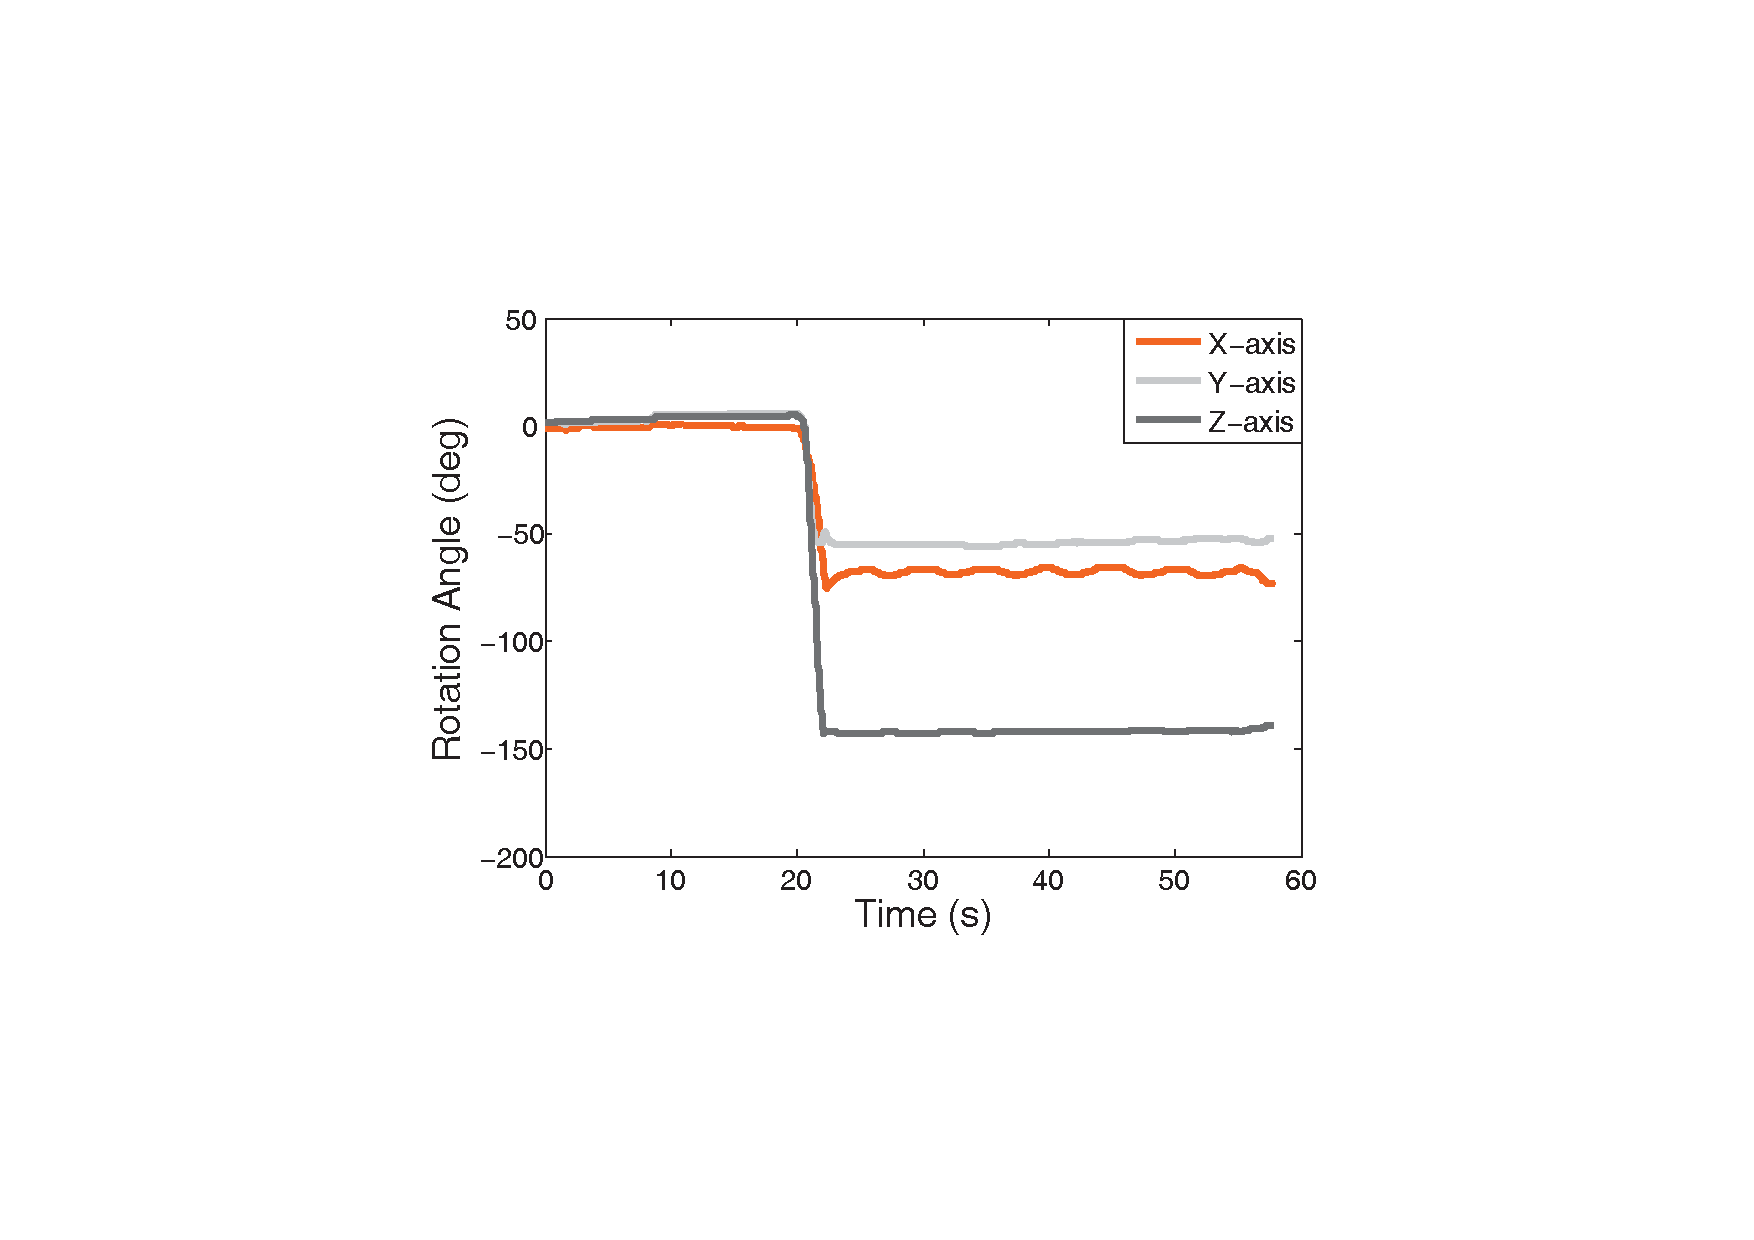
\includegraphics[width=0.32\linewidth]{Figures/BodytoChest.pdf}}
%	%  \hfill
%	\subfigure[]{\label{BodytoShoulder}
%		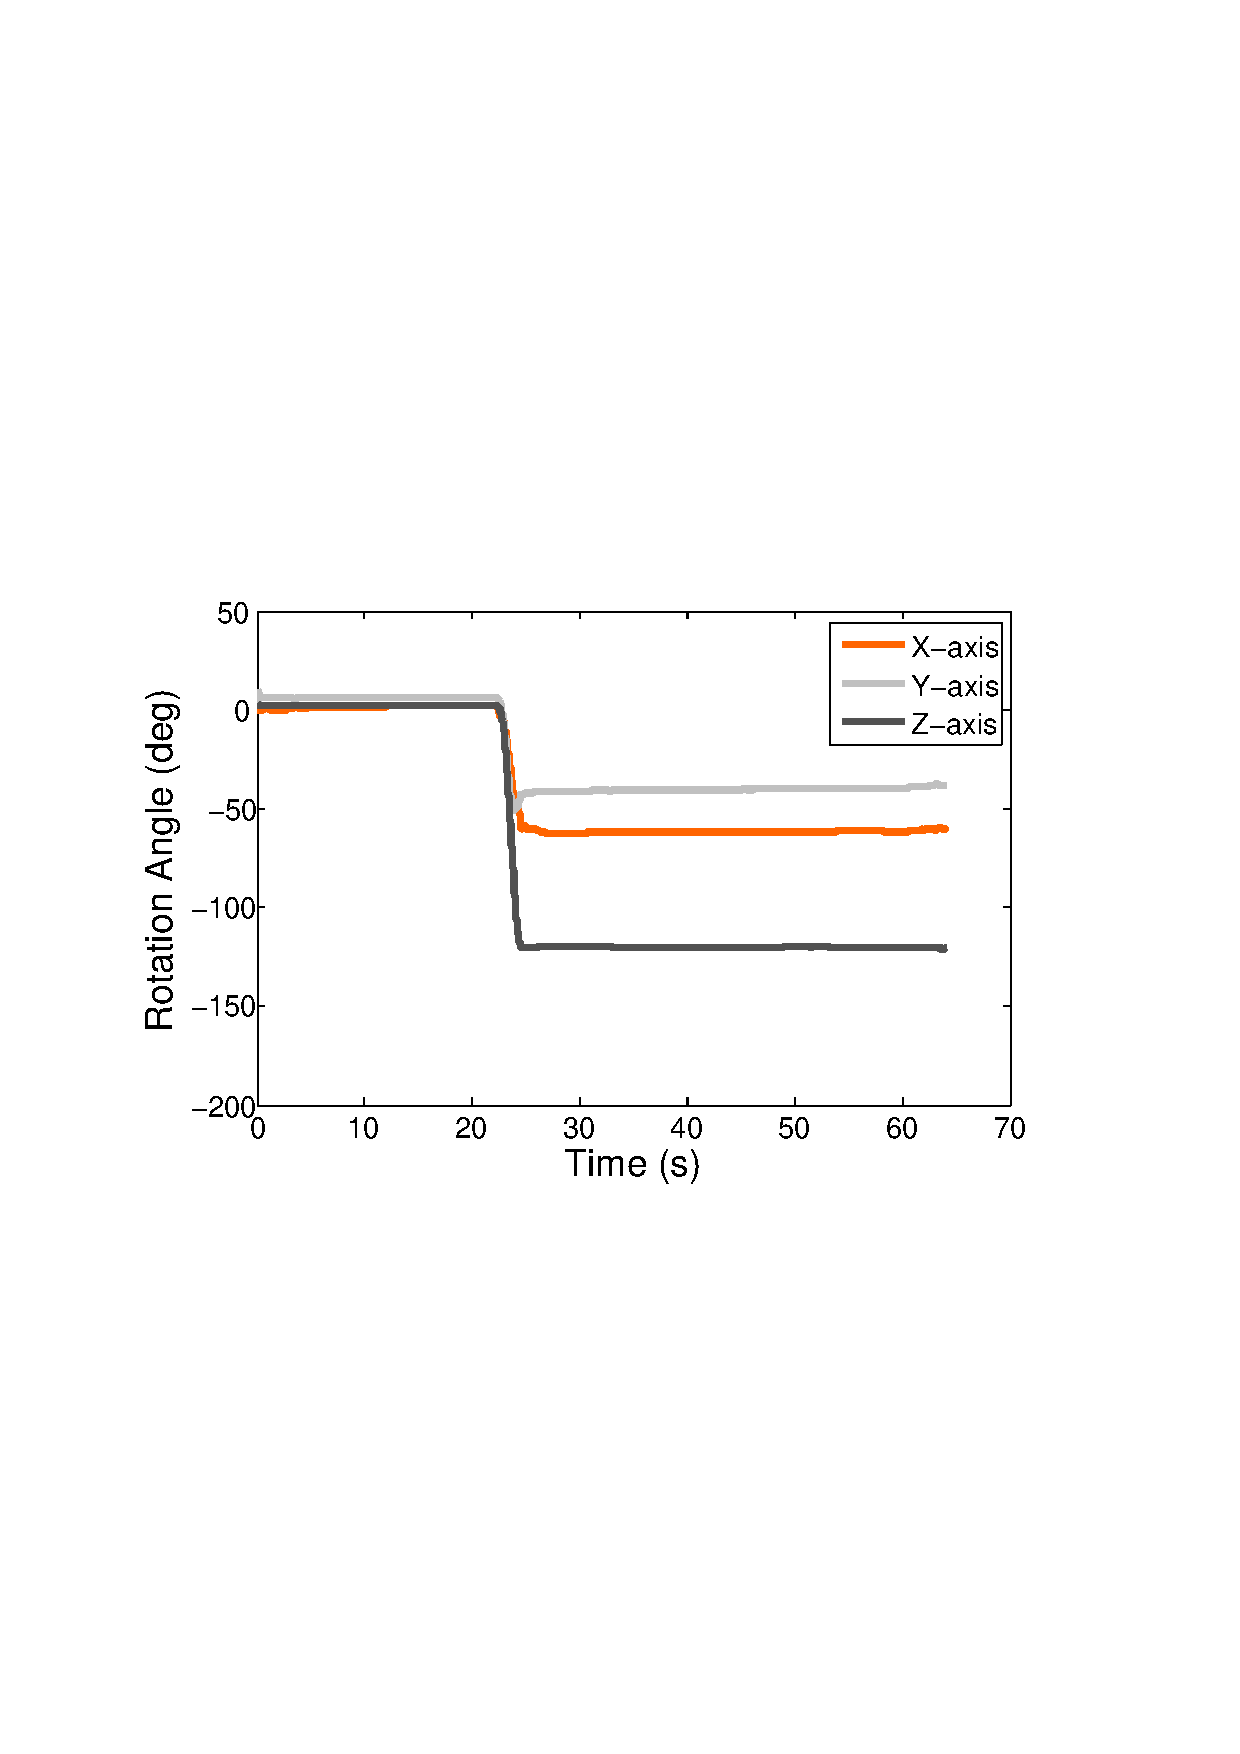
\includegraphics[width=0.34\linewidth]{Figures/BodytoShoulder.pdf}}
%	\caption{The characteristics of hand movement from the position beside the body  to (a)  the chest, and (b) the shoulder.}\label{Bodyhand}
%\end{figure}
%
%\subsection{``Page 9: What is the reasoning behind "if the postures are different, we exclude this time point"? It is possible that a user can have multiple rollover events within a short period.''}
%
%{\bf Response:} Thanks for your comment and we are very sorry that this is a clerical error.
%
%The correct one should be "If the postures are same, we exclude this time point, otherwise the system detects a body rollover event." The resulting large change in angle may be due to the large movement of the arm, so in order to rule out such situations, in addition to calculating the exercise duration, we can use the sleep posture classification algorithm to determine whether the body postures are the same or not over a period of time before and after this point. Also, the user may have a situation where the user turns over continuously for a short period of time. So the angle will change at multiple points in time, we can calculate the body postures over a period of time before and after every point.
%
%\subsection{``Page 9: The parameters of the Moving Average filter need to be introduced.''}
%
%{\bf Response:} Thanks for your valuable comment and we have added the introduction of this parameter in the corresponding part.
%
%The moving average filter is based on the statistical rule, and the length of the moving window we use is 35, which can achieve better filtering effect and will not cause data distortion.
%
%\subsection{``Page 10: Eq. 5 is the first-order derivative of the merged acceleration, which should not be called "acceleration variance".''}
%
%{\bf Response:} Thanks for pointing out this issue and we have modify it.
%
%\subsection{``Page 10: Was the acceleration threshold 0.03 selected on the training data or the test data?''}
%
%{\bf Response:} Thanks for pointing out this issue.
%
%The acceleration threshold 0.03 selected on the training data. In the recognition of the micro body movement, we set an acceleration threshold so as to avoid some tiny body movements are ignored or some acceleration noises are mistaken as body movements. In order to achieve the best detection performance, we try to select an appropriate threshold based on the 100 sets of training data and eventually we set the threshold to be 0.03. And then we have used this acceleration threshold in test data and this value has been proved to be appropriate.
%
%\subsection{``Page 13: Sec. 2.3 introduces a situation where the wrist turned so that the back of the hand become downward, but the situation is not considered in the design of the posture detection algorithm.''}
%
%{\bf Response:} Thanks for pointing out this issue and the valuable comments.
%
%The situation of the wrist turned so that the back of the hand become downward, we considered in the design of the posture detection algorithm. For example, when a user change sleeping posture to the left side, the user��s hand may be close to the pillow with the palm facing up. when sleeping in supine,the user put his hand on the head so the back of user��s hand become downward. Or there is a micro body movement like the hand movement so that the back of the hand become downward.
%
%
%\subsection{``Page 13: There is no standard definition for "light sleep stage" or "deep sleep stage". They need to be defined based on the AASM sleep cycles.''}
%
%{\bf Response:} Thanks for your valuable comments.
%
%We will describe the definition for sleep stage is as follow:
%
%Physiological communities often regard sleep as a cyclical process composed of three stages: rapid eye movement (REM) stage, light sleep stage and deep sleep stage. The biological characteristics of different sleep stages exhibit distinguishingly. In clinical sleep study, the sleep stages are mainly identified by simultaneously evaluating three fundamental measurement modalities including brain activities, eye movements, and muscle contractions. The EEG measure using electrodes placed around the scalp interpret various sleep/wake states of the brain. And, EMG and EOG using electrodes placed on the skin near the eyes and on the muscles, respectively, measures in deeply differentiating REM stage from all the other stages. REM is an active period of sleep marked by intense brain activities and dream occurrence. Light sleep stage is a period of relaxation, when the heartbeat, breathing rate and muscle activity slow down. Deep sleep stage triggers hormones to promote body growth, as well as the repair and restoration of energy. But, apart from the implicit physiological activities, sleepers usually exhibit distinguishable physical activities in different sleep stages. For example, there are somniloquy and body trembles caused by frequent dreams generally appear in REM, large body movements such as body rollovers and arm raising happen in light sleep and micro body movements such as body trembling and snoring occur in deep sleep. Moreover, sleep cycle usually repeats four to six times over a night. The sleeper usually experiences a transition from light sleep to deep sleep and then enters REM, but sometimes there is also possible a phenomenon of skipping some certain sleep stages occurs during sleep. However, despite this, dependence between two successive sleep stages still exists, which also mentioned in SleepHunter.
%
%\subsection{``Page 14: One of the drawbacks of the experimental setup is that the subjects always slept alone. Whether the proposed approach can be generalized to multi-sleeper situations need to be added to the Discussion section.''}
%
%{\bf Response:} Thanks for your valuable comments and we have added this in the Discussion section.
%
%The content we added in the Discussion section of  the revised paper is as follows:
%
%"Currently, {\systemname} considers that the user is sleeping alone, but there are still more complicated situations in reality, such as sleeping with a bed partner, baby, and/or a pet. However, because {\systemname} is based on the detection of smartwatch, Unlike smartphone placed on the bed, it can show more sensitivity to the user's own activities. Therefore, for the detection performance of sleeping posture, body rollover and hand position events has almost no effect, but it may have some influence on the body micro movements and acoustic events. When people around us have relatively large movements, such as body rollover, they may fluctuate to users, making it possible for us to mistakenly detect it as user's micro movements. For this kind of situation, we can test the change of acceleration data in multi-sleeper situations by popularizing the experiment to adjust the detection threshold of our body's micro movements and achieve better detection performance. This will also be a direction for our future work. As for acoustic events, we can further limit conditions, such as training the different magnitudes of the energy of the sound signals collected by the user's hand at different positions to identify whether it is the user's own acoustic event or the sound of the bed partner. In addition, the related acoustic events of the bed partner can also be considered as a factor affecting the user's sleep."
%
%\subsection{``Page 16: Tables need to be self-explained. It should be denoted in Table 3 that the first row is the rollover numbers.''}
%
%{\bf Response:} Thanks for your valuable comments and we have modified it.
%
%
%\subsection{``Page 16: How was the phone accelerometer data labelled for micro body movement detection? Manually?''}
%
%{\bf Response:} Thanks for your question.
%
%Detailed description is as follow:
%
%When assessing the detection accuracy of micro body movement, we use camera to get the ground truth. In the meanwhile, in order to avoid missing some movements such as trembling concealed by the quilt, we also use the accelerometer embedded in the smartphone which placed on the bed to record the occurrence of micro body movements. For the acceleration data collected by smartphone, we first smooth the acceleration along the three axes, calculate Root Sum Square (RSS) to merge them, and obtain the first-order derivative of the merged acceleration. And then we use the threshold detection method to mark the occurrence of motion. Since body trembling is the easiest to be covered, we only focus on such events. So we use smartphone to detect the occurrence of events and the classification of the event is not performed.
%
%\subsection{``Page 19: A correlation analysis is recommended for the results in Table 9.''}
%
%{\bf Response:} Thanks for pointing out this issue and we have added this in the Corresponding part.
%
%The content we added in the revised paper is as follows:
%
%"In Table 9, as we can see, these value are the 14-day average results obtained by combining the sleep quality scores for each participant per day. The scores are divided into four levels, recorded as 0, 1, 2 and 3, representing poor, general, good and excellent, respectively. We compared sleep quality scores from {\systemname}, Fitbit, and user surveys. We can see that although {\systemname}'s assessment of sleep quality scores is only consistent with 9 users' subjective feelings. and only slightly better than Fitbit's results.However, results of the {\systemname} assessment are similar to those of the user survey. Possible inconsistencies are scores 2 and 3, that is, good and excellent, score 0 and 1, that is, poor and general, and there are few cases in which bad sleep has been assessed as good. These similar results are acceptable. We also found that when the results of the {\systemname} were inconsistent with the results of the user survey, it was consistent with the Fitbit results. The reason for such a situation may be that, for example, the user feels good about his own sleep but actually still has some neglected problems during sleep, which is detected by the sleep detection device, which is very helpful to the user."
%
%\subsection{``Page 20: An occurrence probability of unusual arm's positions in the collected data would be useful for the discussion.''}
%
%{\bf Response:} Thanks for your valuable comments and we have added this in the Discussion section.
%
%The content we added in the Discussion section of the revised paper is as follows:
%
%"We detect sleep posture based on arm's positions and focus on three specific positions when detecting the position of the hand. In sleep position detection, we are based on the assumption that between the user's arms position and sleeping postures that the arms have common and (reasonably) stable positions in each posture and we consider as many possible arm positions as possible in four sleeping postures, which are the most common arm's positions for users during sleep. In hand position detection, we chose the three most representative locations that do have an impact on sleep and health. But we know that not all users or a user will not have these common positions all the time. These unusual arm's positions may cause the performance of our sleep posture detection algorithm to degrade. But of the 15 participants we tested, we can see from the video that the unusual arm's positions are present, but these are basically a slight evolution of the common positions, which have little effect on the detection of the sleeping posture. Only a small part of the unusual position will cause us to produce false positives. For this issue, we will expand the test population to further measure the impact of unusual arm's position on our system and consider more hand positions in future work."


%\section{Revision Plan for the Comments of Reviewer 2}
%
%\subsection{``comparison of the measurements of sleep quality and sleep stages with medical grade groundtruth''}
%
%{\bf Response:} Thanks for pointing out this issue and the valuable comments.
%
%We didn't compare our  measurements of sleep quality and sleep stages with medical grade groundtruth. Below we will explain the reasons from two aspects.
%
%Firstly, {\systemname} is a holistic sleep monitoring system based on actigraphy, so its performance on sleep monitoring is not comparable to professional medical equipment like PSG. But compared with PSG or similar scientific methods, {\systemname} concentrates on physical activities rather than biomedical signals, so these rich physical activities detected are easily understood by users, and they can be effectively adjusted and improved sleep based on the results of monitoring. These are more meaningful and more valuable to the ordinary public than complex biological signals and various indicators. Moreover, it does not need special additional devices for detection.
%
%Secondly, we will clarify our groundtruth and the reasons for selecting it.
%When we evaluated the performance of {\systemname} for detecting sleep stages, we chose Fitbit as the groundtruth for the sleep stages. On the one hand, Fitbit is a commercial state-of-the-art and a popular sleep monitoring wristband. It has less interference with the subject's normal sleep process, making easier for subjects to relax and maintain normal sleep, and it is inexpensive and easy to deploy, so it is very convenient to apply to our large number of experimental scenarios. And it shows better performance in this kind of products based on actigraphy. On the other hand, there were some previous work~\cite{fitbit01,fitbit02,fitbit03} demonstrating Fitbit to have a high sensitivity for sleep, good association of movement measurements and to be comparable to PSG in adults. Fitbit is able to adequately track sleep cycles across the night and also can show promise in detecting sleep-wake states and sleep stage composition relative to PSG, particularly in the estimation of REM and light sleep. However, in these related works, it is also pointed out that Fitbit shows some significant limitations that it may overestimate sleep efficiency and total sleep time, so it is not an adequate substitute for PSG. But despite this, for us to use Fitbit to reference REM, light sleep, deep sleep have a minor effect. Moreover, one of the big drawbacks is that the PSG must attach a large number of electrodes and instruments to the subject's body. This will have a certain impact on the subject's psychology and sleep, making the result may do not reflect a real sleep condition. Even if the PSG measurement results are very accurate, the reliability of the data may be reduced due to the intrusiveness to sleep. So for all reasons we use the less intrusive similar product, Fitbit, as the groundtruth of the assessment system, instead of PSG which is expensive, time consuming, intrusive.
%
%
%
%\subsection{``re-framing the paper to make the scientific contribution clear -- so far it is mainly another implementation of a sleep monitoring devices on a similar platform (e.g. similar to fitbit)''}
%
%{\bf Response:} Thanks for the comment.
%
%We first compare {\systemname} with other sleep monitoring system to show our advantages.
%
%In addition to these commercial sleep detection apps or wristbands currently on the market, there are already many scientific works devoted to the study of sleep. Some of them are based on additional hardware devices such as image acquisition devices, pressure mattresses, WISP tags, etc. to infer the user's body position and their movement in the bed. And some of them are based on self-made wearable devices, such as wrist-worn devices, ear-worn devices, etc, to detect changes in sleeping posture or sleep stages. Compared to this type of work, {\systemname} uses only commercially available devices without the need for additional hardware devices and significant changes in people's behavior to detect sleep posture and motion events. Another class of work that is more similar to {\systemname} is based on sensors in smartphones to detect sleep and infer sleep quality. However, many of the work based on the sensors in the smartphone need to ensure that the smartphone is placed on the bed closer to the user, so as to better detect the slight movement of the user's body. However, it is easy to ignore many events that are important and meaningful for sleep assessment, and {\systemname} monitors more meaningful events in the user's actual sleep, such as sleep posture, hand position, breathing amplitude, and more fine-grained body micro movement, and designs a series of interesting algorithms to achieve the recognition and classification of these events. {\systemname} is a more complete system for the use of smartwatch for sleep monitoring. It can not only assess the sleep quality and infer the sleep stage based on these events detected by us, but also provide suggestions for users' bad sleep habits through these rich events, as well as trace back to the real causes affecting sleep quality, and guide users to have the direction to improve sleep quality. Compared with some work based on wearable devices to monitor sleep, {\systemname} is the first holistic sleep monitoring system to rely solely on sensors available in an off-the-shelf smartwatch to capture a wide range of sleep information.  For sleep monitoring in daily life, it is more practical and will not invasion users' normal sleep , and more and more people are willing to accept to wear watches to fall asleep, unlike other wearable devices such as chest-worn sensors, most people are still unwilling to accept to wear her to sleep.
%
%And then from a scientific perspective, our challenge and contribution are listed in detail as follows. And we will elaborate on each of the algorithms we have designed.
%
%\begin{itemize}
%  \item Posture Detection: As we all know, it is very difficult to use only a smartwatch to describe the posture of the entire body, but we found a key basis for sleeping posture detection through observation and a pilot (see Sec. 3 in our paper). The key intuition for distinguishing between these postures is that arms have common and (reasonably) stable positions in each posture. Thus, we can build a mapping between the user's arms position and sleeping postures and identify the user��s posture by identifying periods where the hand is in a position that correlates with a specific posture.
%  \item Hand Position Recognition: The key intuition is that any change in hand position results in a movement trajectory that is uniquely determined by the start and end position of the hand. However, if we only use the hand��s movement trajectory to determine the position of the hand, then we only get the movement relative to a certain known starting position, not the final absolute position of the hand. That is, only when we know that each time the starting position of the hand before movement, we can judge the final hand position based on different trajectories. However, in practical applications, it is difficult for us to obtain the starting position of the hand every time. Therefore, we only cannot rely on the hand movement trajectory to achieve the purpose of detection. However, we found that when the hand is placed on the head, the hand placement is clearly different from that of the hand on the chest or abdomen, which makes it easier to detect by the angle characteristics calculated by the acceleration when placed on the head. When the hand is on the chest or abdomen, the angle characteristics are very similar and difficult to distinguish. Hence, we need an additional verification step to ensure the hand is on the chest or abdomen. We can based on key intuition is that we can observe acceleration signals to exhibit a distinctly periodic fluctuation. This is due to the movement of the abdomen and chest caused by breathing. Therefore, we can use the occurrence of respiratory events to determine if the hand is indeed on the body (abdomen or chest). Through the detection of respiratory events, we can not only determine the initial position of the hand before movement but also filter out some areas near the chest or abdomen, such as the shoulders or hips
%  \item Body rollover counts: The most intuitive way to detect the body rollover events is to detect the direction of rotation of the arm (the rotation angle measured by the gyroscope). However, there is a big drawback to this method. In the actual sleep process, the trajectory of the arm is very difficult to be predicted, especially for different users, and even if there is a slight difference in the starting position of the same sleeping position, it will cause the rotation angle to change and it is easy to cause misjudgment, so this method is not feasible. Therefore, we need to find a feature that is more representative of the body rollover events. And we observe different change patterns about the tilt angle values, when the rollover occurs.Specifcally, the angle values of three different axes are on the falling edge or rising edge simultaneously during a very short time period. To this end, a naive method to detect rollovers would be to rely on changes in angle measurements. However, this method suffers a very large error since other hand movements will also induce a similar change. To deal with this challenge, we incorporate the body postures to improve the detection accuracy. The body postures are different before and after the rollover. Therefore, after we detect the time when the angle values changes, we term the time as a possible rollover time point. And then, we preform the sleep posture detection algorithm to detect sleep posture before and after this point.
%  \item Micro body movement: we can easily divide the body movement events into large movement and micro movement by detecting the signal duration time. In order to distinguish micro-body movements, including hand movement, arm raising and body trembling, it is very intuitive to detect based on the duration of the movement, because we find that the durations of these movements are significantly different. So we try to use the duration of these movements to perform detection. However, we find that the average duration of the arm rising is 1.8 s, but the duration of the other two types of movement is around 1 s, so it is difficult to set a suitable threshold to accurately detect them. Therefore, only through the duration of the movement we can only detect the arm rising with obvious feature. For the hand movement, and body trembling is not effective. However, we have found that body trembling is a sudden movement event, which leads to a more pronounced change in acceleration, so we can use acceleration changes to distinguish them based on such an observed fact.
%  \item Acoustic Event: Different from traditional parameters based on acoustic classification algorithm, which is based on multi-dimensional signal feature extraction methods to detect, which will lead to high complexity of the algorithm. To avoid this problem, we directly perform physical signals detection and recognition by mining the essential characteristics of events. In other words, we exploit the inherent characteristics of different acoustic events and design a lightweight algorithm for effective classification. And then we detect the start and end point of the signal, we improve the traditional algorithm, improving the accuracy of detection and avoiding a large amount of training data.
%  \item In conclusion, We present the design of {\systemname}, the first holistic sleep monitoring system to rely solely on sensors available in an off-the-shelf smartwatch to capture a wide range of sleep information that characterizes overall sleep quality, user behaviours during sleep, and the sleep environment.It can not only assess the user's quality, but also trace back to the real causes affecting sleep quality, and guide users to have the direction to improve sleep quality.
%\end{itemize}
%
%
%
%\subsection{``explaining the long term insight for the scientific community.''}
%
%{\bf Response:} Thanks for the comments.
%
%{\systemname} is the first holistic and a novel smartwatch-based sleep monitoring system that aims at estimating sleep quality and capturing rich information about behaviour and events occurring during sleep. Compare with other sleep detection and quality assessment systems based on actigraphy, our increased detection events include sleep posture, hand position, respiratory amplitude, and body rollover events. Increasing these events in {\systemname} can help us to improve the detection of sleep stage performance and thus better assess sleep quality. But more importantly, it can help users to analyze potential reasons for sleep problems and provide the user with suggestions and directions to improve their sleep habits or sleep environment.
%
%In fact, these events we choose to detect are all related to the quality of sleep and health. For example, improper hand position can even result in health issues, placing the hand on the head can put excess pressure on shoulder nerves and cause arm pain as blood ?ow is restricted. We want to remind users to improve and avoid physical problems by detecting these events that may cause sleep or health problems but are most easily overlooked by people.
%
%So {\systemname} not only provide some novel algorithms to detect these important sleep-related events based on smartwatch, and assess the sleep quality for users, but also help users to find the actual reason of poor sleep quality and make them have a direction to improve sleep quality.



%\section{Revision Plan for the Comments of Reviewer 3}
%
%\subsection{``It is clear that SleepGuard can detect salient aspects of sleep (like sleep position, head position, body rollover etc.), However, it is less clear how this relates to an overall sleep quality measure. While a technical measure of sleep quality is proposed in Section 2.4, the purpose of the User survey in Section 4.2.4 is unclear and results are inconclusive.''}
%
%{\bf Response:} Thanks for the comments.
%
%For the relationship between these events we detected and sleep quality assessment, we elaborated as follows:
%
%{\systemname} is a novel smartwatch-based sleep monitoring system that aims at estimating sleep quality and capturing rich information about behaviour and events occurring during sleep. Compare with other sleep detection and quality assessment systems based on actigraphy, our increased detection events include sleep posture, hand position, and body rollover events, as Table 8. Increasing these events in {\systemname}, on the one hand, can help us better assess sleep quality. On the one hand, it can help users to analyze potential reasons for sleep problems and provide the user with suggestions on how to improve their sleep routine or sleep environment. For evaluating the sleep quality, current commercial actigraphy-based sleep quality assessments device or system is basically based on the occurrence and frequency of body activity and acoustic events during sleep to roughly infer the sleep stage and assess sleep quality, but {\systemname} have made more detailed divisions of body movement events, for example, we considered the occurrence and frequency of body rollover events, three kinds of different micro movements, and the amplitude of respiratory. These more fine-grained events can more accurately represent different stages of sleep. This is due to the fact that there are significant differences in the types of physical activity and respiratory amplitude at different stages of sleep. And according to our investigation and previous research works, the quality of sleep is largely determined by the percentage of different sleep stages during the whole sleep process. So more accurate detection of sleep stages is achieved through more extensive event detection. It helps provide better decision support for evaluating the sleep quality.
%
%
%And there are two purposes for which we conduct user surveys. And the specific explanations are as follows:
%
%On the one hand, in order to verify the effectiveness of {\systemname}, we conducted a comprehensive assessment of the performance of the system; on the other hand, in order to understand and verify whether the events detected by {\systemname} are really interested or needed by users, we investigated and researched users. The user survey we conducted consisted of two types of people. One is the 15 volunteers who participated in our experiment, we not only conducted a sleep quality assessment for them but also investigated these users' experience for {\systemname}. And the others do not use our system, so, they only be asked if they were interested in or recognized the events we detected. Therefore, the results of the user survey are also composed of two parts. They are the assessment of sleep quality and the survey of user experience.For the assessment of sleep quality, we ask users to fill in questionnaires based on PSQI to get the user's subjective feelings, and compare the results of {\systemname} and Fitbit measurements with it. In Table 9, these values are the 14-day average results obtained by combining the sleep quality scores for each participant per day. The scores are divided into four levels, recorded as 0, 1, 2 and 3, represent poor, general, good And excellent, respectively. We can see from the table that although {\systemname}'s assessment of sleep quality scores is only consistent with 9 users' subjective feelings. and only slightly better than Fitbit's results, we can find that even the results from {\systemname} are different from the results from the user survey, but the levels are close. For example, there is a user has a score of 3, representing excellent, and a score of 2 is shown in the evaluation result of {\systemname}, which means that the quality of sleep is good. These similar results are acceptable, and there are few cases in which bad sleep has been assessed as good. And, basically, when the user feels bad sleep quality, {\systemname} can also accurately detect it. For the user experience, we can find that most people are praised and interested in these events detected by {\systemname}. Moreover, we also asked 15 participants who participated in the assessment of sleep quality to adjust themselves based on the recommendations made by {\systemname} and investigate them after 3 weeks. It was found that some of the users had some symptoms relieved and the average quality of sleep was improved. We can see that the improvement is still satisfactory.
%
%\subsection{``provide evidence that the detailed measures provided by SleepGuard can be used to improve sleep quality (beyond what current systems provide)''}
%
%{\bf Response:} Thanks for the comments.
%
%We will clarify the advantage of {\systemname} in helping users improve sleep quality, mainly from the original intentions of the events we selected, the detailed description of user survey and the analysis of the results of our user survey.
%
%In fact, these events we choose to detect are all related to the quality of sleep and health. For example, improper hand position can even result in health issues, placing the hand on the head can put excess pressure on shoulder nerves and cause arm pain as blood ?ow is restricted. We want to remind users to improve and avoid physical problems by detecting these events that may cause sleep or health problems but are most easily overlooked by people.
%
%And we can also find through the user survey these sleep behaviour we detected are indeed effective and beneficial for people, especially for users with sleep problems.The user survey we conducted consisted of two types of people. One is the 15 volunteers who participated in our experiment, we not only conducted a sleep quality assessment for them but also investigated these users' experience for {\systemname}. And the others do not use our system, so, they only be asked if they were interested in or recognized the events we detected. 80\% of participants believe that the detection of sleep posture is very necessary, showing their sleep posture can not only help people to avoid health problems caused by long-term improper sleeping posture, but also help us find out the reasons for the next day's physical discomfort, such as dizziness, muscle soreness may be due to improper sleeping posture. And there are some users are troubled by snoring. This may be due to improper sleeping posture. We map the detected snoring event and sleeping posture to suggest the user to modify his posture to a suitable posture to reduce the harm caused by long-term snoring. 60\% of the participants thought it useful to detect the hand position in supine posture, even one user mentioned that he did often have nightmares and our system found his hand was often placed on his chest, and then {\systemname} could remind him that he should take some measures to avoid such a position and thus reduce the poor sleep quality that nightmare brings.
%
%In addition, we summarized the sleep problems and habit of the 15 volunteers who participated in our system assessment through a questionnaire survey and quality of sleep assessment. Then we found that there are a participant reported that his arm was always paralyzed, and five participants had poor sleep quality. We can find that the reason why the user's arm is numb is his incorrect sleep habits. The results from SleepGuard showed that he always tends to put his hands on his head, and long-term postures like this will inevitably lead to numbness of the arms. For similar situations, we will inform and remind users of their inappropriate postures and habits, and recommend that users should take measures to improve such situations. And for the poor quality of sleep of users, we analyzed the cause one by one based on events detected by {\systemname}. Through {\systemname}'s detecting, one user showed obvious symptoms of the difficulty of falling asleep and an unusually high number of body rollover. Our further analysis revealed that there was excessive light intensity and frequent noise in his sleeping environment. This may have led to the appearance of these symptoms and thus the poor quality of sleep. Then {\systemname} will recommend that users should focus on and improve his sleeping environment. In fact, this situation is very common that some users often choose to sleeping with a bright light because of one's fear of going to sleep alone. Even if they can also feel that this has an impact on their sleep. But in fact doing so for a long time is very bad for sleep and health. So {\systemname} also gives some suggestions for resolution, for example, do some proper exercise before going to bed or go to sleep with soft music that can be automatically turned off. And there is a user reported that he always had a nightmare at night, which led to poor sleep quality. We analyse the results of {\systemname} and found that user has been accustomed to sleep in the left side, and sometimes the hand is habitually placed on the chest. As \cite{nightmare} points that people who sleep on their left side are more at risk of nightmares. And the oppression of the chest by the hand causes the brain to have an ill hallucination, making it extremely easy to make a nightmare. So {\systemname} suggest to the user based on these two possible reasons, and hope that the user can take some special measures to change it, and recommend that the user can take some additional methods, such as listening to some soothing music to relax before sleep. Another user was detected by {\systemname} to be bothered by long-term snoring, as he himself mentioned. We know that the occurrence of snoring is most likely due to improper sleeping posture, and we also detected that the user is accustomed to sleep in a supine position, so on the one hand, {\systemname} suggests that the user try the sleeping position in the side position. On the other hand, if the situation still does not improve very well, it is recommended that the user go to the hospital in time for a corresponding check to avoid snoring caused by certain diseases. In addition, if we detect that some users are accustomed to sleeping in a prone position, we will remind and advise them because the prone position is bad for health.
%
%According to these different possible reasons, {\systemname} proposes different reminders and suggestions to users, such as adjusting their sleeping posture, improving the sleeping environment, and consciously avoiding bad sleeping habits. And it is recommended that long-term snoring users perform physical examination so that they can timely The discovery of physical diseases that is most likely to cause snoring such as high blood pressure, cardiovascular and cerebrovascular diseases. In addition, we asked the 15 participants to make appropriate adjustments according to our recommendations and to conduct a return visit survey three weeks later. It was found that some of the users had some symptoms relieved and the average quality of sleep was improved. Therefore, we can find that, on the one hand,  {\systemname} detect these rich, fine-grained sleep-related events is effective, on the other hand it can really help users to find the cause of poor sleep quality and give users the direction and reference to improve sleep quality.
%
%\subsection{``provide evidence that SleepGuard is able to provide sleep insights beyond what is provided by current commercial or research systems.''}
%
%{\bf Response:} Thanks for the comments.
%
%Sleep monitoring provided by current commercial or research systems is mainly divided into two categories: one is similar to PSG based on various physiological signals, such as brain waves, electrocardiogram. The other is based on actigraphy-based systems mainly implemented on the smartphone or wristband. {\systemname} is a holistic sleep monitoring system belonging to the second categorie. Although the accuracy of sleep monitoring is not as high as this type of system compared to the first type of system, {\systemname}'s accuracy is sufficient for the general public's sleep monitoring needs in daily life and we concentrates on physical activities rather than biomedical signals, so these rich physical activities detected are easily understood by users, and they can be adjusted with improved and improved sleep based on the results of monitoring. These are more meaningful and more valuable to the ordinary public than complex biological signals and various indicators, it does not need special additional devices for detection. Compared with some existing commercial devices or research based on actigraphy, the performance of {\systemname} has been improved to some extent, but more advantages are reflected in the consideration of more abundant events. Our original intention and focus are more inclined to enable users to have a deeper and more comprehensive understanding of their sleep, explore the cause s of sleep quality, and provide users with more practical advice to point them in a clear direction for improving sleep quality and being healthy.

%\section{Revision Plan for the Comments of Reviewer 5}

%\subsection{``Is this a right way to capture sleep related events? What are the limitations of using a single wrist sensor to capture sleep related behaviors accurately?''}
%
%{\bf Response:} Thanks for your valuable comment.
%
%In our paper, we only use the sensor data in the left-hand smart watch, though movement patterns of the left and right wrist are different during sleep, the technique used for detecting sleep related behaviors is the same. Some sleep related events like sleep posture, body rollover, acoustic events, illumination conditions, both of them are not affected by different wrists, the only thing we need to do is adjusting new experimental parameters when the smartwatch is worn on different wrists. But for the hand position detection and body micro movement detection including the arm raising and hand movement does have an impact, and the degree of impact on our detection performance varies from person to person. This is where we need to measure and consider in our future work.
%
%\subsection{``how does this system help users to improve sleep quality? In other words, if users noticed that they have specific sleep posture, hand posture or roll over often, how can he/she change the behaviors/posture?''}
%
%{\bf Response:} Thanks for your valuable comment.
%
%We have detected richer sleep-related events than existing sleep detection systems.  It can not only assess the sleep quality and infer the sleep stage based on these events detected by us, but also provide suggestions for users' bad sleep habits through these rich events, as well as trace back to the real causes affecting sleep quality, and guide users to have the direction to improve sleep quality.
%
%Specifically, according to different possible reasons, {\systemname} proposes different reminders and suggestions to users, such as adjusting their sleeping posture, improving the sleeping environment, and consciously avoiding bad sleeping habits. And it is recommended that long-term snoring users perform physical examination so that they can timely The discovery of physical diseases that is most likely to cause snoring such as high blood pressure, cardiovascular and cerebrovascular diseases. We only provide users with a suggestion for different reasons. The user can take some medical measures or special methods according to their own situation to change the sleeping posture or hand position.
%
%
%\subsection{``It was not clear that the ground truth the authors used was validated or whether we can reply on them.''}
%
%{\bf Response:} Thanks for your valuable comment and we have further to clarify.
%
%When we evaluated the performance of {\systemname} for detecting sleep stages, we chose Fitbit as the groundtruth for the sleep stages. On the one hand, Fitbit is a commercial state-of-the-art and a popular sleep monitoring wristband. It has less interference with the subject's normal sleep process, making easier for subjects to relax and maintain normal sleep, and it is inexpensive and easy to deploy, so it is very convenient to apply to our large number of experimental scenarios. And it shows better performance in this kind of products based on actigraphy. On the other hand, there were some previous work~\cite{fitbit01,fitbit02,fitbit03} demonstrating Fitbit to have a high sensitivity for sleep, good association of movement measurements and to be comparable to PSG in adults. Fitbit is able to adequately track sleep cycles across the night and also can show promise in detecting sleep-wake states and sleep stage composition relative to PSG, particularly in the estimation of REM and light sleep. However, in these related works, it is also pointed out that Fitbit shows some significant limitations that it may overestimate sleep efficiency and total sleep time, so it is not an adequate substitute for PSG. But despite this, for us to use Fitbit to reference REM, light sleep, deep sleep have a minor effect. Moreover, one of the big drawbacks is that the PSG must attach a large number of electrodes and instruments to the subject's body. This will have a certain impact on the subject's psychology and sleep, making the result may do not reflect a real sleep condition. Even if the PSG measurement results are very accurate, the reliability of the data may be reduced due to the intrusiveness to sleep. So for all reasons we use the less intrusive similar product, Fitbit, as the groundtruth of the assessment system, instead of PSG which is expensive, time consuming, intrusive.

%\subsection{``I think tracking the detailed sleep behaviors using a wrist sensor is interesting but this topic itself is not novel. There is some prior work that captures sleep posture and sleep related information using wrist sensors. The authors need to explain how the proposed methods are different from previous ones and why the proposed methods are better.''}
%
%{\bf Response:} Thanks for your valuable comment.
%
%Compared with some existing commercial devices or research based on actigraphy, {\systemname} is a more complete sleep monitoring system,
%and is based only on sensors in commercial smart watches without additional hardware. For sleep monitoring in daily life, it is more
%practical and will not invasion users' normal sleep , and more and more people are willing to accept to wear watches to fall asleep, unlike
%other wearable devices such as chest-worn sensors, most people are still unwilling to accept to wear her to sleep. And the performance of
%{\systemname} has been improved to some extent, but more advantages are reflected in the consideration of more abundant events. Our
%original intention and focus are more inclined to enable users to have a deeper and more comprehensive understanding of their sleep,
%explore the causes of sleep quality, and provide users with more practical advice to point them in a clear direction for improving sleep
%quality and being healthy.


 %\subsection{``2.1 Posture Detection: Hands can be all over the place with 4 sleep body postures and could be rotated in different ways, then this looks like hand posture detection rather than body posture detection.''}
%
%{\bf Response:} Thanks for your valuable comment.
%
%When a user sleeps in different positions, his hand (arm) is normally at different positions with different postures, and the arms position and pose are related to the body position. Take the left arm as an example: when sleeping in supine, the user is likely to put his hand on the left side of the body, on the abdomen, on the chest or on the head; when sleeping on left, the user is likely to put his hand close to the pillow with the palm facing up. Based on this observation, we can see that there is a mapping between the user's arms position and sleeping postures that the arms have common and (reasonably) stable positions in each posture. Thus, we can identify the user��s posture by identifying periods where the hand is in a position that correlates with a specific posture. And we also try to consider more possible positions of the arms in each sleeping position to improve the effectiveness of sleep position detection.

%\subsection{``Hand Position Detection: Why don't we have "others"? Can we also we breathing frequency to identify sleep stages?''}
%
%{\bf Response:} Thanks for your valuable comment.
%
%We considered three hand positions, that are on the abdomen, chest or head when the user is in the supine posture. Our reason for choosing these three positions is that they are representative. They are the most common hand position in the supine position and have some influence on sleep and health. For example, placing the hand on the head can put excess pressure on shoulder nerves and cause arm pain as blood flow is restricted.
%
%
%In fact, the difference in respiratory amplitude will also affect the difference in respiratory frequency, because when the respiratory amplitude is large, the time taken for one breath will be long, and the frequency of breathing will be slower. Therefore, respiratory frequency can also be used as a feature of sleep stage detection. In our paper, we choose the respiratory amplitude because the feature is very intuitive, but their essence is the same.


%\subsection{``Hand Position Detection: A method to evaluate a hand position classifier lacks detailed information.''}
%
%{\bf Response:} Thanks for your valuable comment.
%
%The rotation angle changes when the hand is moving from an initial point beside the body to different positions on the body. So we use the three-axis rotation angle calculated by the gyroscope as a feature to train a classifier based on the template distance matching.


%\subsection{``Hand Position Detection: What are larger respiratory amplitude and normal respiratory amplitude? How were the data labeled? Which classifier was used?''}
%
%{\bf Response:} Thanks for your valuable comment.
%
%Based on previous studies and our observations, we can know that when people sleep in the REM stage, their respiratory amplitude is smaller than in the other stages. The level of minute ventilation in rapid-eye-movement (REM) sleep (6.46 $\pm$ 0.29 l/min) being significantly lower than in non-REM sleep (7.18 $\pm$ 0.39 l/min). In this paper, we define the more pronounced chest undulation, ie, breathing during the NREM phase, as large respiratory. And we consider respiratory during the REM phase as normal respiratory.
%
%Therefore, we combined the sleep stage with the acceleration variance for getting the threshold of the large respiratory and normal respiratory. Specifically, We trained a classifier using this feature when the hand is placed on the abdomen and on the chest under both REM stage and NREM stages to determine a mapping from current respiratory amplitude to placement. As for the acquisition of sleep stage, we use the intersection of the {\systemname} and Fitbit measurement results. When the sleep stages measured by the {\systemname} and Fitbit are consistent, ie REM or NREM, we determine that the current sleep stage is REM or NREM. The threshold of respiratory-induced acceleration variance is trained at different stages, but it is of course only effective if the hand is in the chest and abdomen. At the same time, We also take into account video recorded by the camera to manually label part of the respiratory. The combination of these three kinds of equipment can enable us to obtain real and accurate data as much as possible. We build a classifier to try to establish a mapping between the amplitude of respiratory and the variance of the acceleration. And we use a template-based distance matching approach to get the two threshold of acceleration variance.

%\subsection{``Body rollover counts: What "if the postures are different, we exclude this time point" mean?''}
%
%{\bf Response:} Thanks for your comment and we are very sorry that this is a clerical error.
%
%The correct one should be "If the postures are same, we exclude this time point, otherwise the system detects a body rollover event." The resulting large change in angle may be due to the large movement of the arm, so in order to rule out such situations, in addition to calculating the exercise duration, we can use the sleep posture classification algorithm to determine whether the body postures are the same or not over a period of time before and after this point. Also, the user may have a situation where the user turns over continuously for a short period of time. So the angle will change at multiple points in time, we can calculate the body postures over a period of time before and after every point.
%
%\subsection{``Acoustic feature calculation: what are x and w in equation 7? Were the proposed method (showed in equations 9-12) better than traditional algorithm? How were equations 11 and 12 built?''}
%
%{\bf Response:} Thanks for your comment.
%
%Equation 7 is the short-term average energy used to calculate the sound signal, where $N$ is the length of the window, $x$ is the signal and $\omega$ is the impulse response, and the short-term energy is the weighted sum of squares of a frame of sample values. Specifically, when the window function is a rectangular window, the equation can be changed to the following form:
%\begin{equation}
%  E_i=\sum\nolimits_{j=i-(N-1)}^{i}x(j)^2,
%\end{equation}
%
%The traditional algorithm uses a fixed double threshold and must be obtained by a large number of data samples, and the fixed double threshold may cause error detection at the beginning of the acoustic event. But our method does not require pre-sampling learning to obtain the threshold parameters. Instead, it utilizes the information of each signal to be detected to perform threshold estimation, which not only reduces the costs of learning but also leads to higher detection accuracy. For each signal to be detected��we select the first five frames and the last five frames of the signal and calculate their features to estimate the background noise. And we combine the short-term energy of noise ($E_n$) and the maximum value of the short-term energy over all frames to get the average short-term energy of the signal ($DE$). Then we can get the adaptive double threshold, as shown in equations 11 and 12.
%
%As for equations 11 and 12, to set the energy threshold for detecting the start and end points of the speech signal, we first need to consider that this threshold must be greater than the energy of the noise signal ($E_n$) to ensure that the noise is filtered out, as shown in the following equation. And then we used the nighttime sound data of 10 volunteers who participated in training to train the multiplier factor of the energy value DE of the speech signal throughout the frame: $\alpha$ and $\beta$. We vary $\alpha$ from 0.1 to 0.5 and $\beta$ from 0.01 to 0.07, eventually set
%$\alpha$ to be 0.1 and $\beta$ to be 0.06, which achieves the best detection performance.
%\begin{equation}
%      EH=\alpha \times DE+E_n,
%\end{equation}
%\begin{equation}
%    EL=\beta \times DE+E_n,
%\end{equation}


%\subsection{``2.3 Illumination Condition: Is there any reason you used 10 lux as a threshold? How do prior studies using actigraphy to measure light use the light reading from the wrist in order to solve a issue about the unstable readings?''}
%
%{\bf Response:} Thanks for your comment.
%
%Our threshold selection is based on experiments. Specifically, we visit 10 volunteers' bedroom at night and the use of the ambient light sensor to test the lighting conditions in the bedroom, and we find that in the absence of light in the bedroom, the reading of the light sensor is basically maintained at 1Lux to 4Lux. In some cases, the watch's screen is awakened and lighted up to cause the light to rise to 4Lux; when the bedroom is in a faint light, such as a table lamp light, the light sensor's average readings are also maintained below 10Lux, so divide the illumination intensity into two conditions: bedroom without light (Weak illumination condition, $\leq$10 Lux); bedroom with strong lights (Strong illumination condition, $>$10 Lux)
%
%Currently, we have not found a study on smartwatch to solve an issue about the unstable readings of the light sensor, but there is a study have mentioned the problem of readings if the light sensors on smartphone are blocked. In Sleep Hunter, they build a light-weight hierarchical illumination intensity sensing scheme. It employs the proximity sensor to detect whether the light sensor is blocked or not. if the light sensor is blocked, then Sleep Hunter locates the latest record of the illumination condition when the light sensor is not blocked, and treats it as the current illumination condition until the light sensor recovers.
%
%Their method is to solve this problem only through the proximity sensor in the smartphone, but it does not apply in smartwatch because there is no proximity sensor. Therefore, we determine whether the light sensor is obscured based on the detection of the wrist movement. If the light sensor is obscured, we use the average of the previous light intensity as the intensity of the time period.

%\subsection{``2.4 Sleep stage and quality Which features were used for sleep stage and quality detection? What is time window length?''}
%
%{\bf Response:} Thanks for your comment.
%
%We build a Hidden Markov Model and use a series of sleep events as the observed sequence and the sleep stage as the implicit stage sequence. $obs_t={NB(t),NB_M(t),BA(t),NA(t)}$ represents the feature vector at detection phase t. The explanation of each item, which is the input of HMM, is listed as follows. $NB(t)$: the number of occurrences of body rollover during the detection phase t. $NB_M(t)$: the number of occurrences of micro body movement. $BA(t)$: the measurement of  respiratory amplitude. $NA(t)$:the number of occurrences acoustic events. And $states_t$ =$\{$light sleep; deep sleep; REM$\}$ is an output of our model, which represents the sleep stage in the detection phase t. And sleep quality is calculated by the proportion of different sleep stages in the entire sleep period, as shown in equation 13 in our paper.
%
%As for the time window length, we use event-driven detection. When there is no sleep event in 15 minutes, we perform a sleep stage detection. When an event occurs, we immediately perform a sleep stage detection and use this time as the starting point for the next 15 minutes.
%

%\subsection{``3.1 What is the sampling rate of sensor measurement on the smartwatch.''}
%
%{\bf Response:} Thanks for this comment and we have added it in the corresponding part.
%
%The data is collected every 30 ms on the smartwatch, which is approximately 33Hz. Although our sampling rate is not very high, it is sufficient for detecting the sleep-related events and this can save energy consumption of the watch compared to a high sampling rate.
%
%
%\subsection{``3.2 Are these 15 volunteers independent from 10 participants who joined a study to validate sleep-related events?''}
%
%{\bf Response:} Thanks for this comment.
%
%These 10 participants were used to train the parameters of each algorithm in the system and the HMM model. They were different from the 15 volunteers who participated in the system assessment and validation.

%\subsection{``3.3 There is another study to validate sleep stage detection from Fitbit Charge2. Can you say this is accurate?''}
%
%{\bf Response:} Thanks for your comment.
%
%When we evaluated the performance of {\systemname} for detecting sleep stages, we chose Fitbit as the groundtruth for the sleep stages. On the one hand, Fitbit is a commercial state-of-the-art and a popular sleep monitoring wristband. It has less interference with the subject's normal sleep process, making easier for subjects to relax and maintain normal sleep, and it is inexpensive and easy to deploy, so it is very convenient to apply to our large number of experimental scenarios. And it shows better performance in this kind of products based on actigraphy. On the other hand, there were some previous work~\cite{fitbit01,fitbit02,fitbit03} demonstrating Fitbit to have a high sensitivity for sleep, good association of movement measurements and to be comparable to PSG in adults. Fitbit is able to adequately track sleep cycles across the night and also can show promise in detecting sleep-wake states and sleep stage composition relative to PSG, particularly in the estimation of REM and light sleep. However, in these related works, it is also pointed out that Fitbit shows some significant limitations that it may overestimate sleep efficiency and total sleep time, so it is not an adequate substitute for PSG. But despite this, for us to use Fitbit to reference REM, light sleep, deep sleep have a minor effect. Moreover, one of the big drawbacks is that the PSG must attach a large number of electrodes and instruments to the subject's body. This will have a certain impact on the subject's psychology and sleep, making the result may do not reflect a real sleep condition. Even if the PSG measurement results are very accurate, the reliability of the data may be reduced due to the intrusiveness to sleep. So for all reasons we use the less intrusive similar product, Fitbit, as the groundtruth of the assessment system, instead of PSG which is expensive, time consuming, intrusive.

%\subsection{``3.3 Participants wear Fitbit Charge2 and the other Smartwatch on a different wrist. Do you think you get different measurement from left and right wrists? Were Sleep Hunter and Sleep as Android validated?''}
%
%{\bf Response:} Thanks for your comment.
%
%In our paper, we only use the sensor data in the left-hand smart watch, though movement patterns of the left and right wrist are different during sleep, the technique used for detecting sleep related behaviors is the same.
%
%We will explain the detailed reason from the fundamental of {\systemname} and Fitbit.
%
%Both Fitbit and {\systemname} have common grounds for detecting sleep stages based on acoustic events, the occurrence and frequency of physical activity, but we go further to conduct more fine-grained detection and classification of these events, and add more consideration about illumination conditions and respiratory amplitude. One thing we can know is that the measurement of events such as acoustic events, body rollover events, body tremble, etc., has little to do with the sensor data collected from the left or right hand. The reason is that these events are related to the entire body rather than the part of the body. The major difference that may exist is these rich events added in {\systemname}, such as hand position, sleep posture, etc, and the only thing we need to do is adjusting new experimental parameters when the smartwatch is worn on different wrists, but these are not detected by Fitbit, so they have no effect when compared. Moreover, we also did a test experiment. The smart watches were worn on the left and right hands respectively and the event detection algorithm in {\systemname} was mainly used to detect those events that are of concern in Fitbit. We can see that the results are not much different. Therefore, in the end, in order to ensure that the user's sleep is as uncomfortable as possible, we choose to make Fitbit and Smartwatch are worn on different hands.
%
%Sleep Hunter and Sleep as Android are  based on the sensors in the smartphone on the bed to detect sleep-related events, so they are not affected by different wrists, and  we did not consider them on this issue.


%\subsection{``4 It was not clear which window length was used for annotating events.''}
%
%{\bf Response:} Thanks for your comment and we have further to clarify.
%
%{\systemname} starts tracking sleep events when it detects that the light is off and there has been no body movement for 30 minutes. As part of an initialization process, {\systemname} estimates the initial body posture and hand position. It then uses these as a starting point to monitor sleep events like the body posture, rollovers, hand positions and body movements. So we use event-driven detection. When there is no sleep event in 15 minutes, we perform a sleep stage detection. When an event occurs, we immediately perform a sleep stage detection and use this time as the starting point for the next 15 minutes.
%
%\subsection{``4.1.1 What is "a modified cross-validation"? Is SleepMonitor validated as well? Why did the authors choose only one participant show the performance of body posture detection?''}
%
%{\bf Response:} Thanks for your comment and we have further to clarify.
%
% Cross-validation refers to taking out most of the samples in a given modeling sample to build a model, leaving a small part of the sample to be forecasted using the newly established model. This process continues until all the samples are predicted once and only once predicted. But our approach is that each time we select one user's data to train the classifier and the rest fourteen users's data to test. This process continues until fifteen users' data are predicted once and only once predicted. So we consider this approach as a modified cross-validation. Using our method can not only achieve the purpose of cross-validation, that is, the results are more fair and reliable, but also get results  in a shorter time, reduce the time cost. And we can also find that using only one person's data to train The classifier is sufficient to achieve good results. So we consider this approach as a modified cross-validation.
%
% As for SleepMonitor, we did not use the cross-validation method to verify it. We only compared the results mentioned in its paper. We found that our sleeping position detection performance is slightly better than that of the SleepMonitor. This may because consideration in our algorithm for more possible arm's positions, covering more possibilities and avoiding the influence of some unusual positions on the detection algorithm.
%
%And the reason why we choose only one participant show the performance of body posture detection is that we have determined through experiments. When we are training the classifier, we first try to train the classifier with one user's data, and we find that using only one user's data can achieve good detection performance. And in order to evaluate performance more effectively, we use a cross-validation method.
%
%\subsection{``4.1.5 The authors say "pre-defined parameters in the detection model does not include all possible patterns. Individual differences in cough patterns can be predictive in advance. Was there anything to do to solve this issue?''}
%
%{\bf Response:} Thanks for your comment.
%
%As we can see from the detection results, the precision for cough event is a little than others. The reason is that different user's cough patterns are different, for example, some people have a fast and continuous pattern of coughing, while others have a slower intermittent pattern. However, our algorithm is based on the characteristics of different acoustic events, so the characteristics of the patterns describing the events need to be obtained through training. We can further expand the training data to include more possible patterns, and can also make reasonable estimates of the possible patterns to refine the range of parameters and thus increase the accuracy.
%
%\subsection{``4.2.4 Are values in Table 9 the mean of measurement over 14 days? "SleepGuard was able to remind him to avoid such as hand position"
%  Is this something users can change?''}
%
%{\bf Response:} Thanks for your comment.
%
%Every morning, we record the sleep quality scores obtained from {\systemname} and Fitbit, and ask these participates to give a sleep quality score according to their own subjective feelings. In Table 9, these value are the 14-day average results obtained by combining the sleep quality scores for each participant per day.
%
%{\systemname} is based on assessed sleep quality to trace the true causes that affect it, then we only provide users with a suggestion for different reasons. The user can take some medical measures or special methods according to their own situation to change their bad sleep habits, such as hand position.
%
%\subsection{``Table 8 is located really far from where it is referred. Shouldn't it be Table 1?''}
%
%{\bf Response:} Thanks for this comment.
%
%We are very sorry for such a wrong mark, and we have already corrected it.

\bibliographystyle{ieeetr}
\bibliography{SleepGuard_Response}
\end{document}
